\documentclass[a4paper,11pt]{ltjsarticle}

% ========== package ========== %
% --- 数式環境 --- %
\usepackage{amsmath}
\usepackage{amssymb}
\usepackage{mathtools}
% --- 数式環境 END --- %
% ブラケット
\usepackage{braket}
% ベクトルの太文字
\usepackage{bm}
% 添え字左右上下 \fourIdx{左上}{左下}{右上}{右下}{ベース} で使う．Iは大文字
\usepackage{fouridx}
% 色
\usepackage{color}
% 余白指定
\usepackage{geometry}
% --- ページ内リンク --- %
\usepackage{hyperref}
\hypersetup{colorlinks=true,linkcolor=blue}
% --- ページ内リンク END --- %
% 花文字
\usepackage{mathrsfs}
% 画像
\usepackage{graphicx}
% tcolorbox
\usepackage{tcolorbox}
% appendix
\usepackage{appendix}
% --- 参考文献 --- %
\usepackage{etoolbox}
\usepackage{fontspec} % fontspecは読み込んでOKですが、設定順序に注意が必要です
%% --- 参考文献フォント --- %%
  \IfFontExistsTF{Times New Roman}{
    \newfontfamily\bibfontface[Ligatures=TeX]{Times New Roman}
  }{
    \newfontfamily\bibfontface[Ligatures=TeX]{FreeSerif} % 代替フォント
  }
%% --- 参考文献フォント END --- %%
%% --- 参考文献リンク位置 --- %%
  \BeforeBeginEnvironment{thebibliography}{%
    \phantomsection
    \addcontentsline{toc}{section}{参考文献}
  }
  \AtBeginEnvironment{thebibliography}{%
    \normalfont\bibfontface
  }
%% --- 参考文献のリンク位置 --- %%
% --- 参考文献 END --- %
% ========== package END ========== %

% ========== newcommand ========== %
% --- セクションから目次へのリンク --- %
\newcommand{\sectionlink}[1]{\section[#1]{\hyperlink{toc}{#1}}}
\newcommand{\subsectionlink}[1]{\subsection[#1]{\hyperlink{toc}{#1}}}
% セクション番号リンク
\makeatletter
\renewcommand{\@seccntformat}[1]{%
  \protect\hyperlink{toc}{\csname the#1\endcsname}\quad
}
\makeatother

\numberwithin{equation}{section}
% ==========- newcommand END ========== %
\allowdisplaybreaks
%===========================================================
% --- タイトル --- %
%===========================================================
\geometry{left=25mm, right=25mm, top=30mm, bottom=30mm}
\usepackage{needspace}
\widowpenalty=10000\clubpenalty=10000

% Section-only translation: retain source numbers and template layout.
\setlength{\emergencystretch}{2em}
\hypersetup{unicode=true,pdftitle={Lectures on Inflation §3.5 日本語訳},pdfauthor={Leonardo Senatore（原著）}}
\makeatletter
\newcommand{\OriginalEquation}[1]{%
  \par\addvspace{7pt}\noindent\begin{minipage}{\linewidth}%
  \def\@currentlabel{#1}\phantomsection\label{eq:#1}%
  \centering\csname eq#1\endcsname
  \end{minipage}\par\addvspace{7pt}}
\makeatother
\newcommand{\OriginalFigure}[1]{\par\begingroup\centering\csname fig#1\endcsname\par\endgroup}
\newcommand{\trnote}[1]{\par\noindent{\small 訳注：#1}\par}
\expandafter\def\csname eq151\endcsname{\makebox[\linewidth][r]{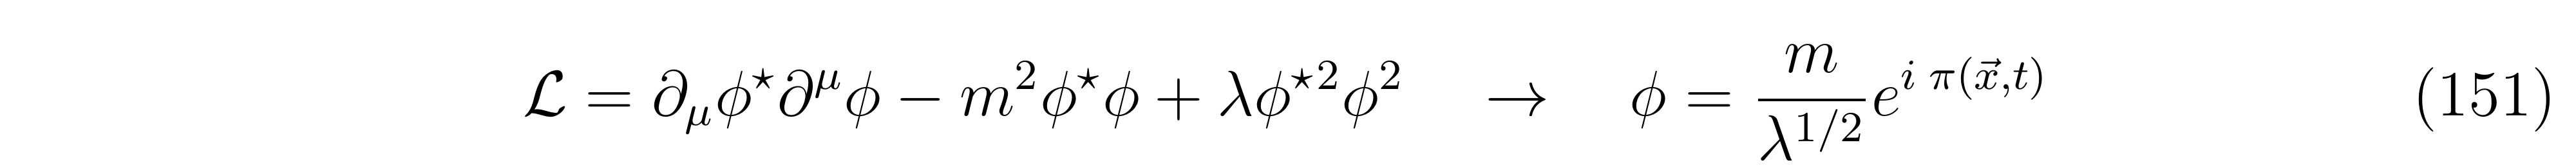
\includegraphics[width=1.000000\linewidth]{assets/eq151.png}}}
\expandafter\def\csname eq152\endcsname{\makebox[\linewidth][r]{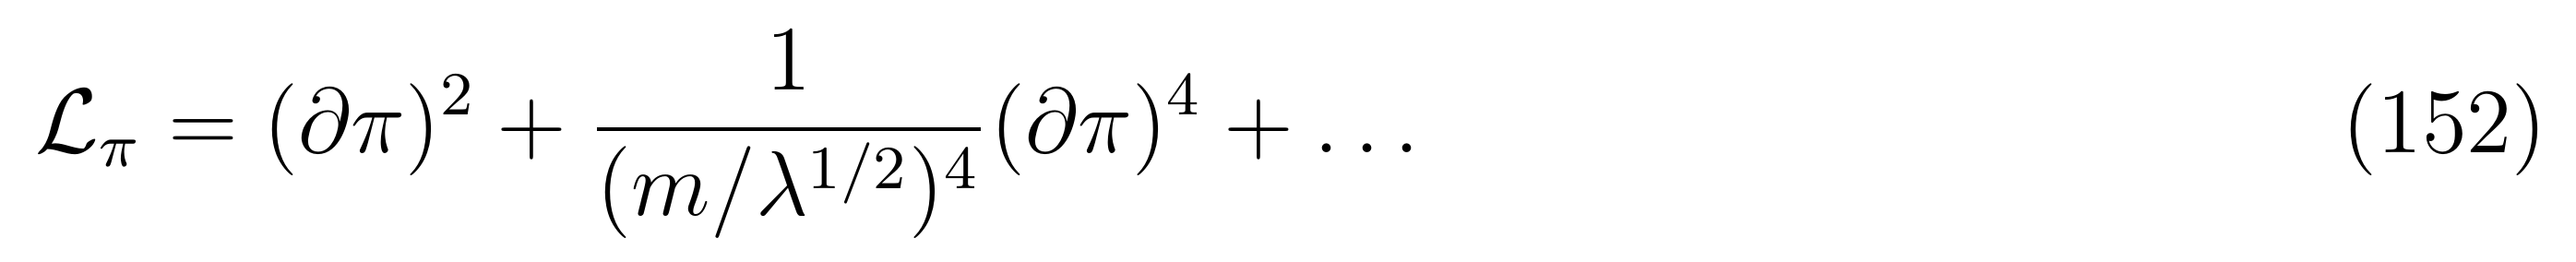
\includegraphics[width=0.697917\linewidth]{assets/eq152.png}}}
\expandafter\def\csname eq153\endcsname{\makebox[\linewidth][r]{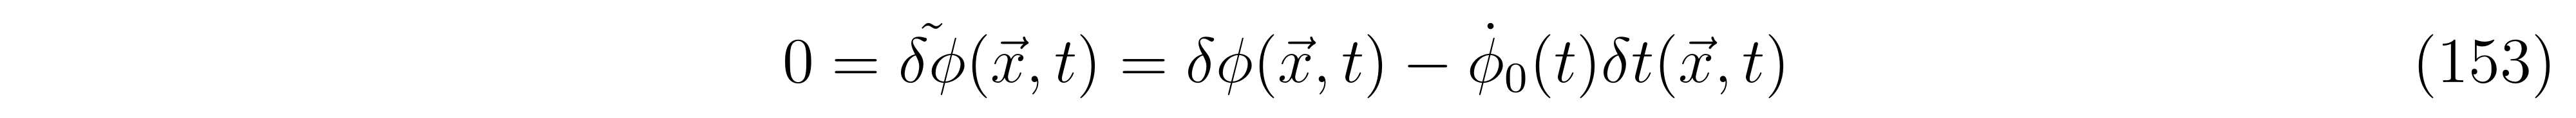
\includegraphics[width=1.000000\linewidth]{assets/eq153.png}}}
\expandafter\def\csname eq154\endcsname{\makebox[\linewidth][r]{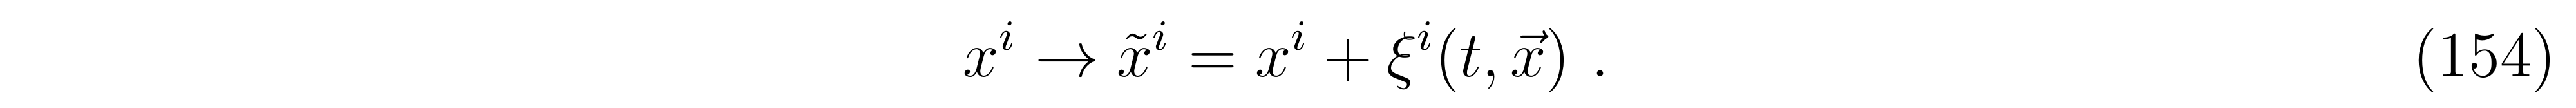
\includegraphics[width=1.000000\linewidth]{assets/eq154.png}}}
\expandafter\def\csname eq155\endcsname{\makebox[\linewidth][r]{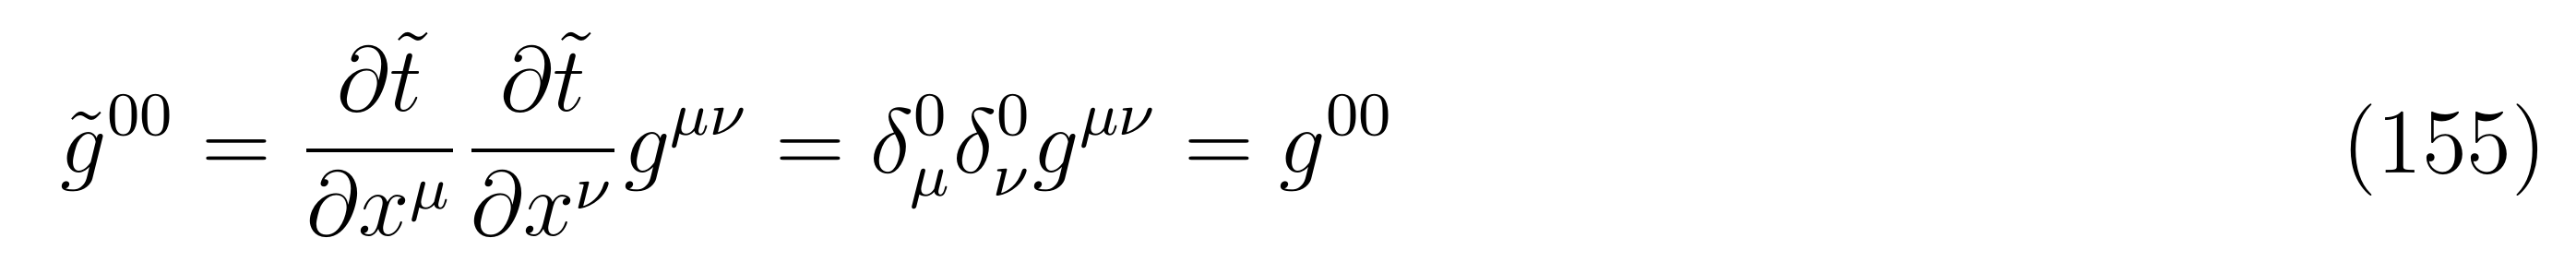
\includegraphics[width=0.697917\linewidth]{assets/eq155.png}}}
\expandafter\def\csname eq156\endcsname{\makebox[\linewidth][r]{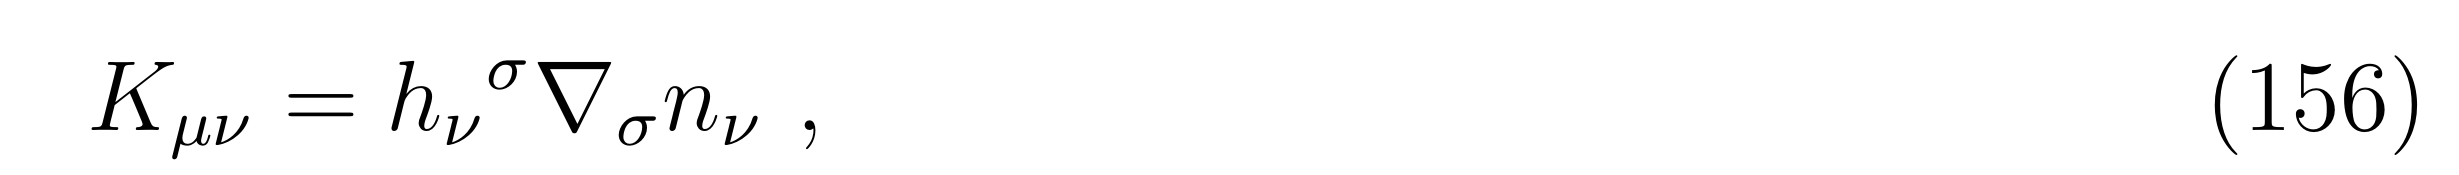
\includegraphics[width=0.614583\linewidth]{assets/eq156.png}}}
\expandafter\def\csname eq157\endcsname{\makebox[\linewidth][r]{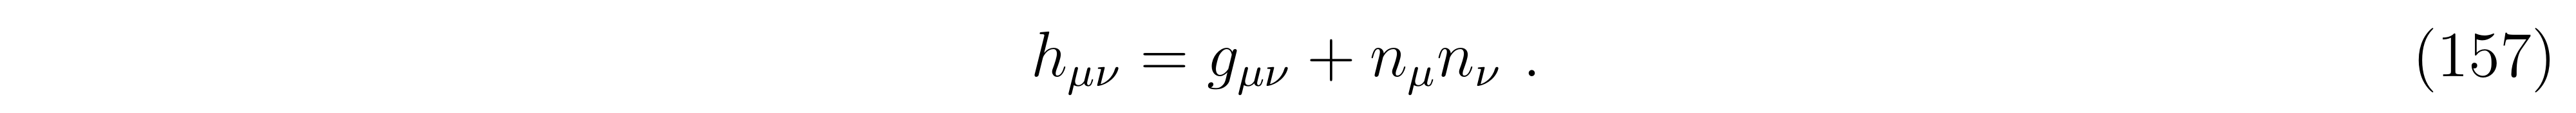
\includegraphics[width=1.000000\linewidth]{assets/eq157.png}}}
\expandafter\def\csname eq158\endcsname{\makebox[\linewidth][r]{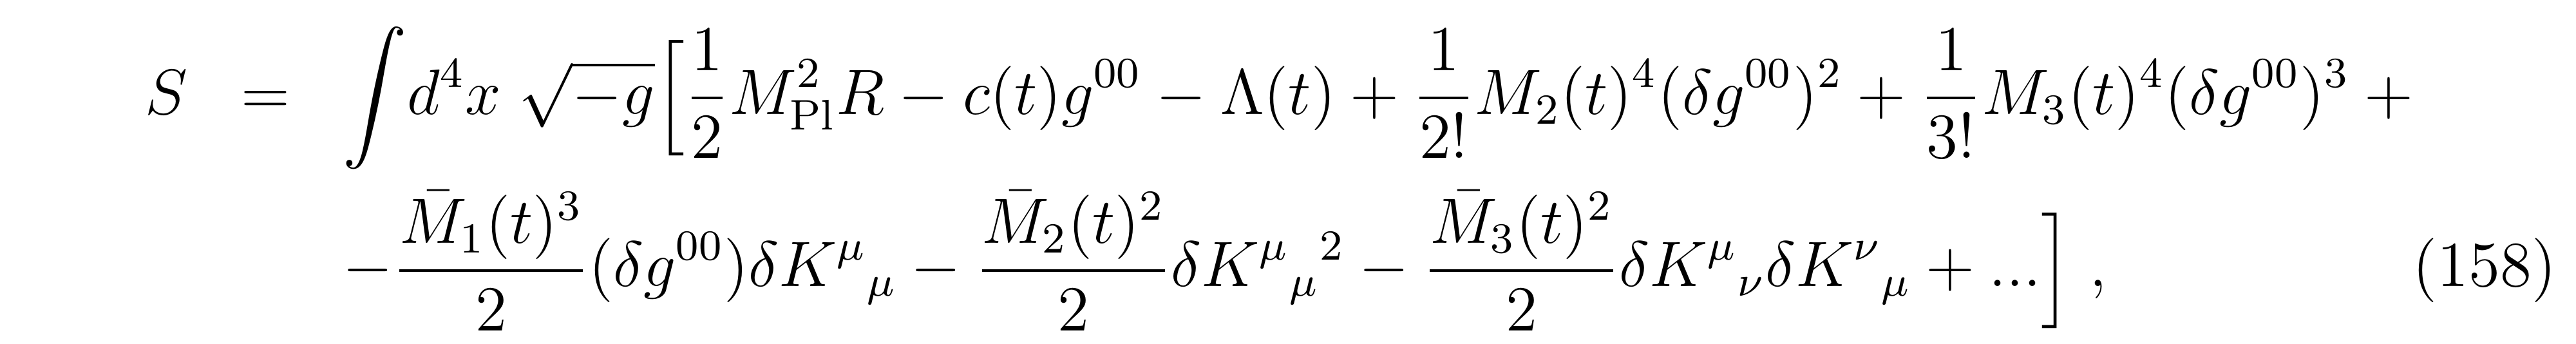
\includegraphics[width=1.000000\linewidth]{assets/eq158.png}}}
\expandafter\def\csname eq159\endcsname{\makebox[\linewidth][r]{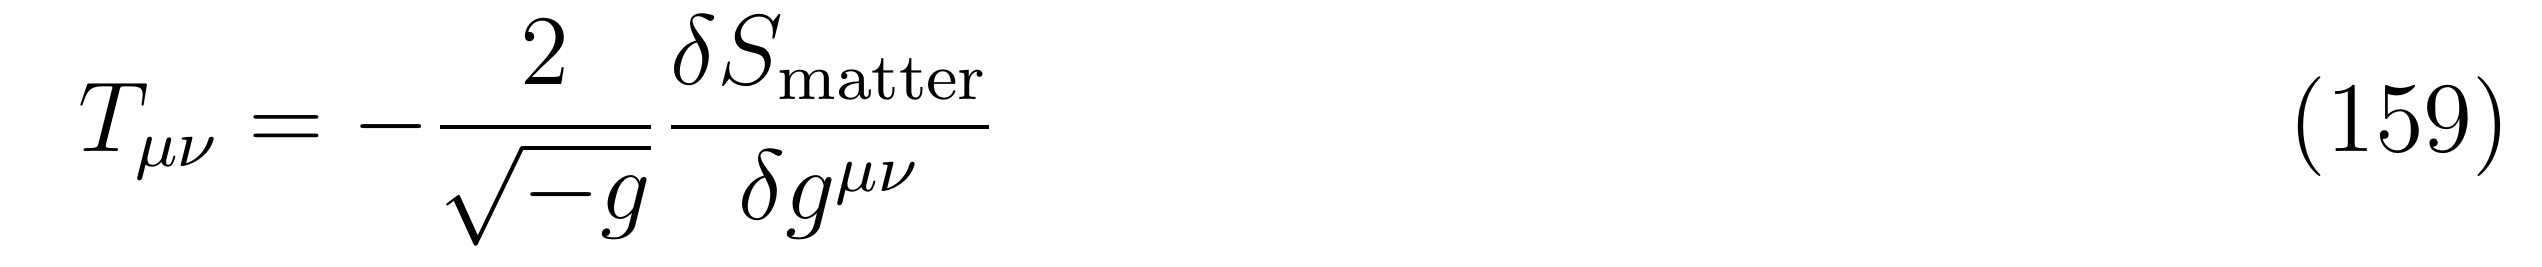
\includegraphics[width=0.635417\linewidth]{assets/eq159.png}}}
\expandafter\def\csname eq160\endcsname{\makebox[\linewidth][r]{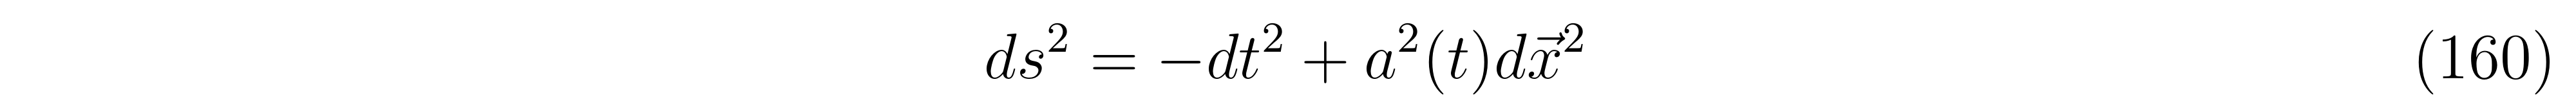
\includegraphics[width=1.000000\linewidth]{assets/eq160.png}}}
\expandafter\def\csname eq161\endcsname{\makebox[\linewidth][r]{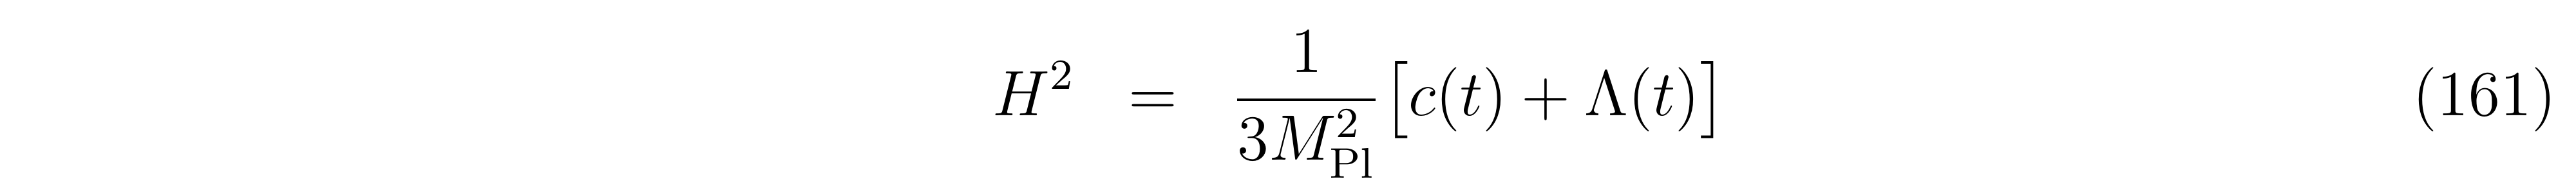
\includegraphics[width=1.000000\linewidth]{assets/eq161.png}}}
\expandafter\def\csname eq162\endcsname{\makebox[\linewidth][r]{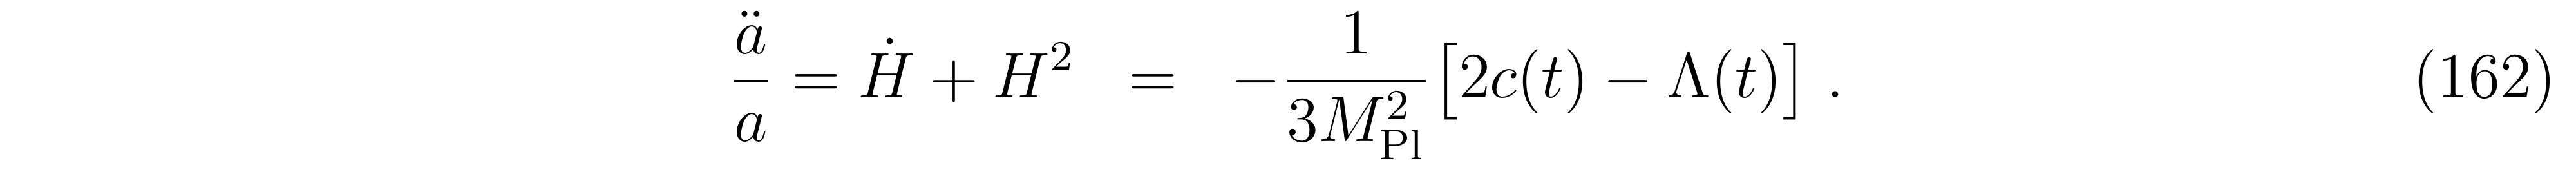
\includegraphics[width=1.000000\linewidth]{assets/eq162.png}}}
\expandafter\def\csname eq163\endcsname{\makebox[\linewidth][r]{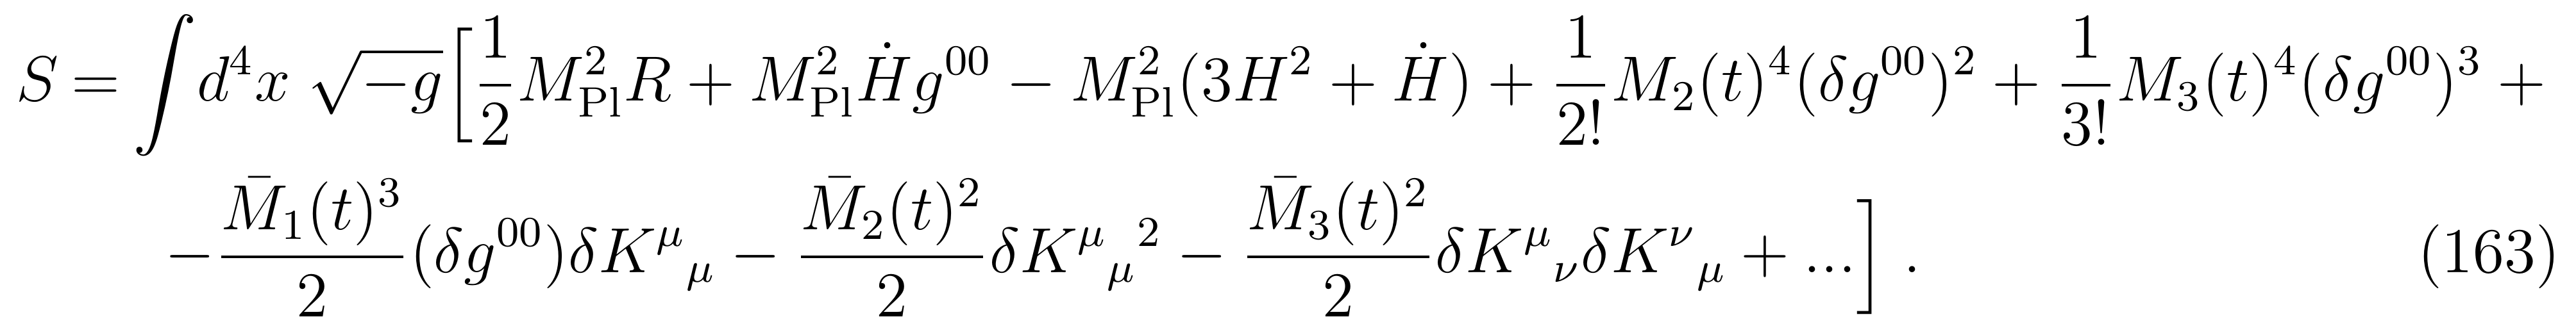
\includegraphics[width=1.000000\linewidth]{assets/eq163.png}}}
\expandafter\def\csname eq164\endcsname{\makebox[\linewidth][r]{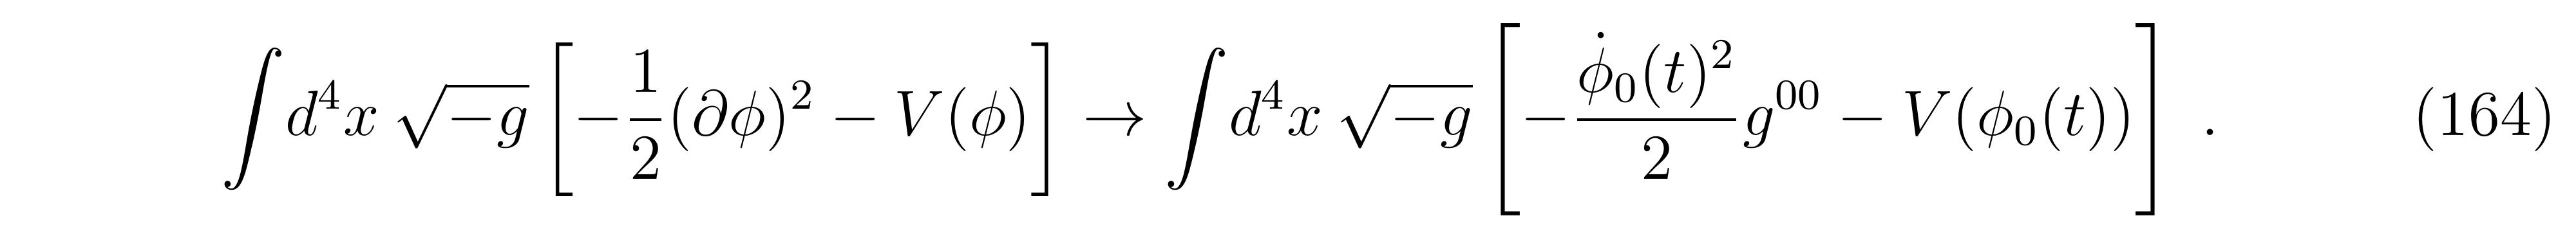
\includegraphics[width=1.000000\linewidth]{assets/eq164.png}}}
\expandafter\def\csname eq165\endcsname{\makebox[\linewidth][r]{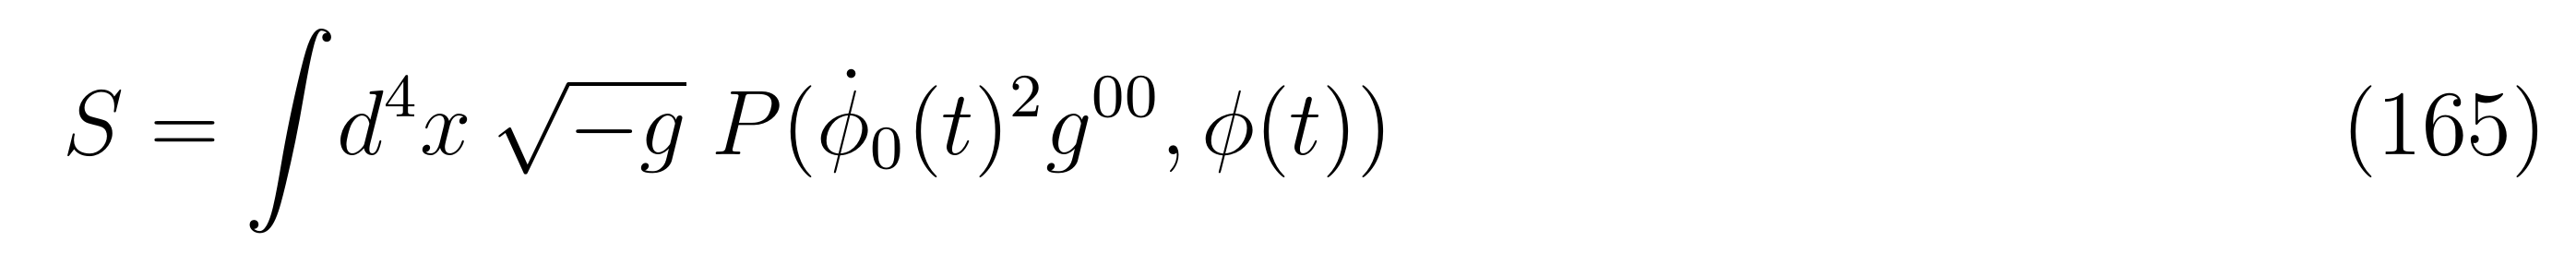
\includegraphics[width=0.697917\linewidth]{assets/eq165.png}}}
\expandafter\def\csname eq166\endcsname{\makebox[\linewidth][r]{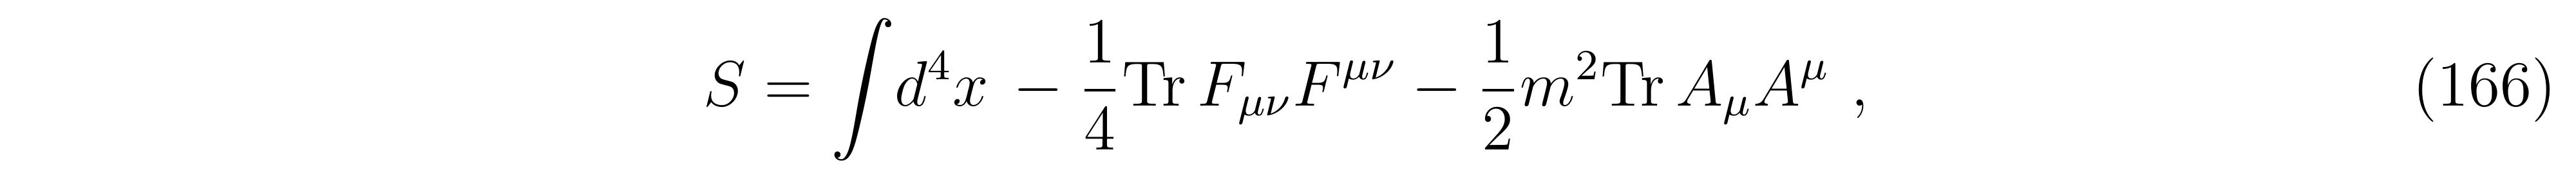
\includegraphics[width=1.000000\linewidth]{assets/eq166.png}}}
\expandafter\def\csname eq167\endcsname{\makebox[\linewidth][r]{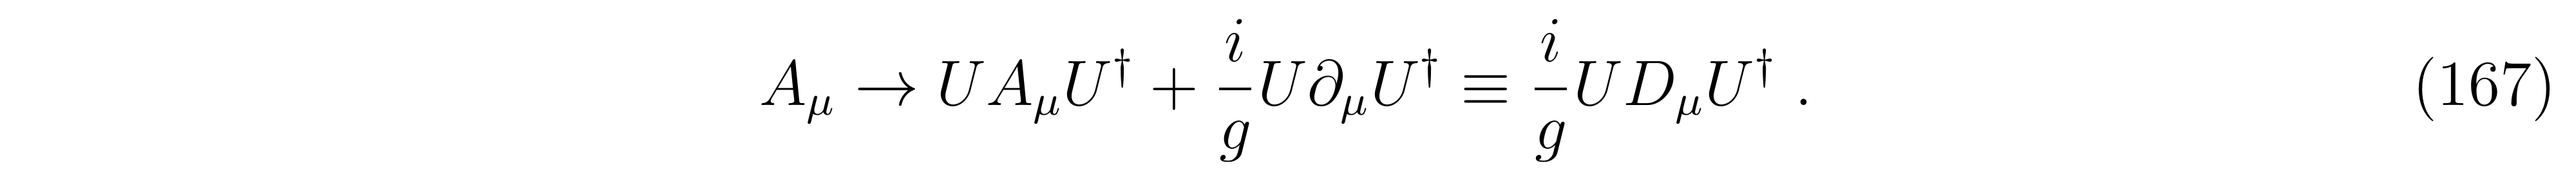
\includegraphics[width=1.000000\linewidth]{assets/eq167.png}}}
\expandafter\def\csname eq168\endcsname{\makebox[\linewidth][r]{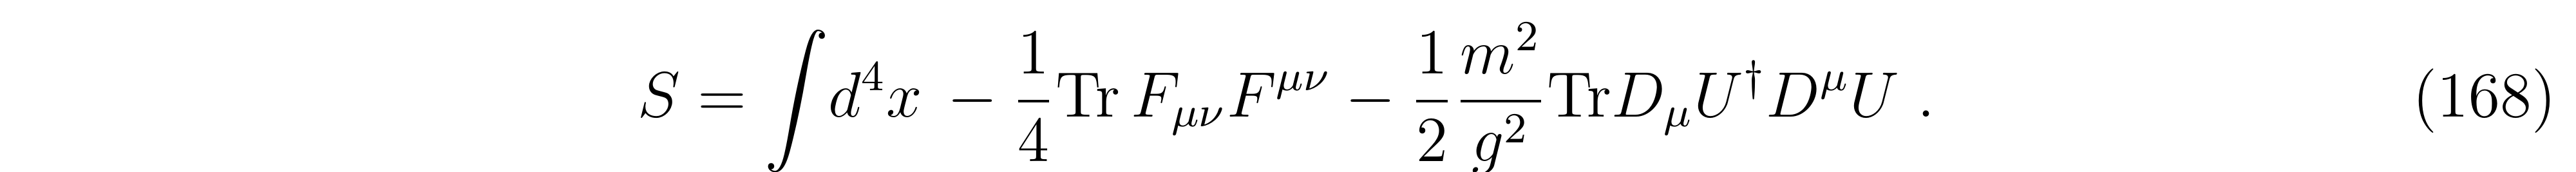
\includegraphics[width=1.000000\linewidth]{assets/eq168.png}}}
\expandafter\def\csname eq169\endcsname{\makebox[\linewidth][r]{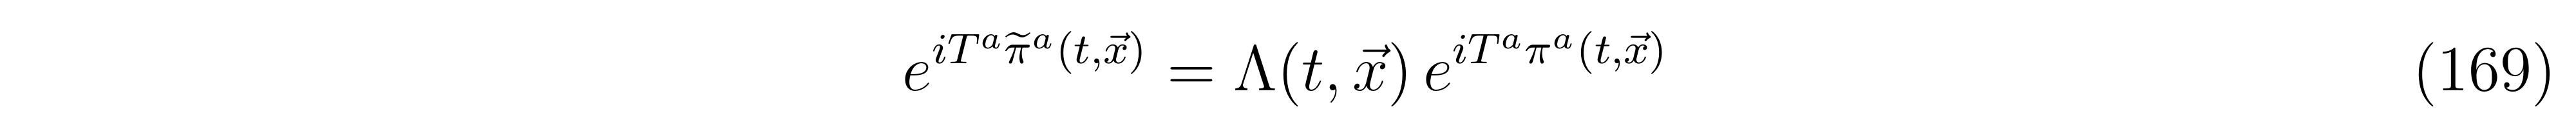
\includegraphics[width=1.000000\linewidth]{assets/eq169.png}}}
\expandafter\def\csname eq170\endcsname{\makebox[\linewidth][r]{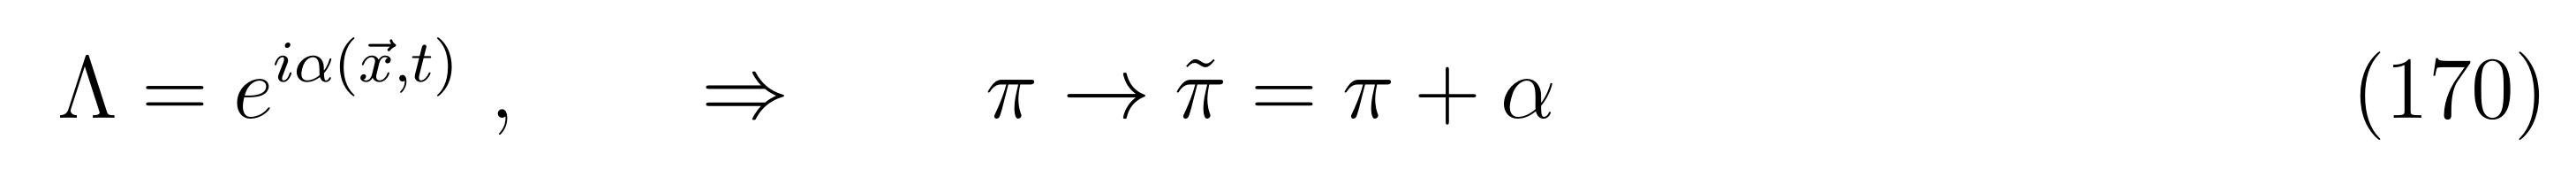
\includegraphics[width=0.729167\linewidth]{assets/eq170.png}}}
\expandafter\def\csname eq171\endcsname{\makebox[\linewidth][r]{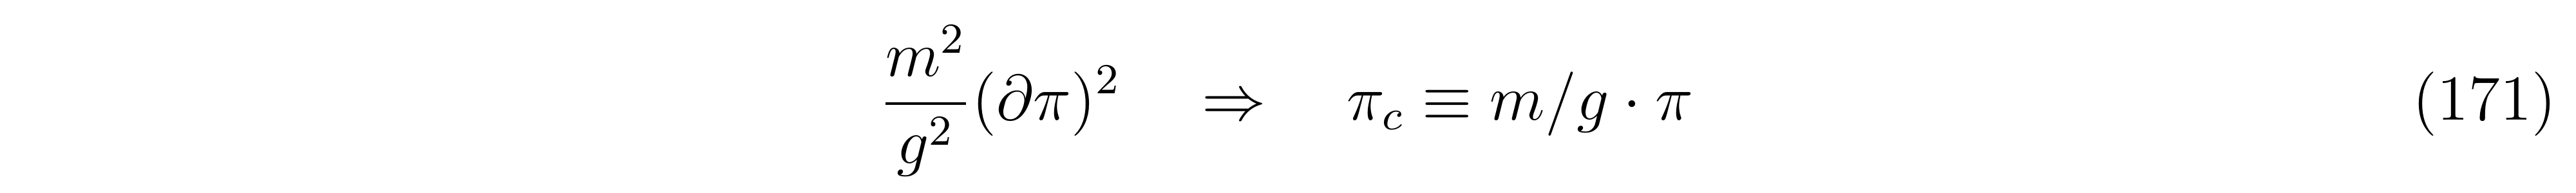
\includegraphics[width=1.000000\linewidth]{assets/eq171.png}}}
\expandafter\def\csname eq172\endcsname{\makebox[\linewidth][r]{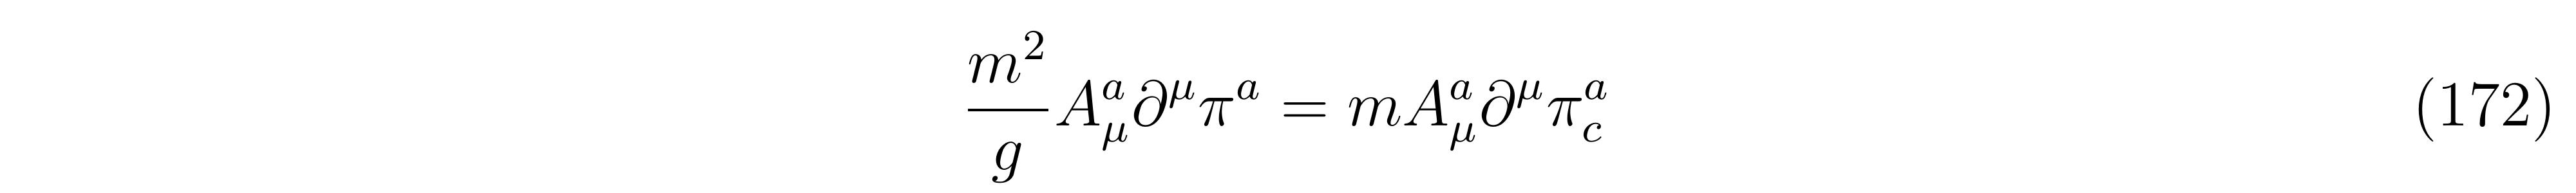
\includegraphics[width=1.000000\linewidth]{assets/eq172.png}}}
\expandafter\def\csname eq173\endcsname{\makebox[\linewidth][r]{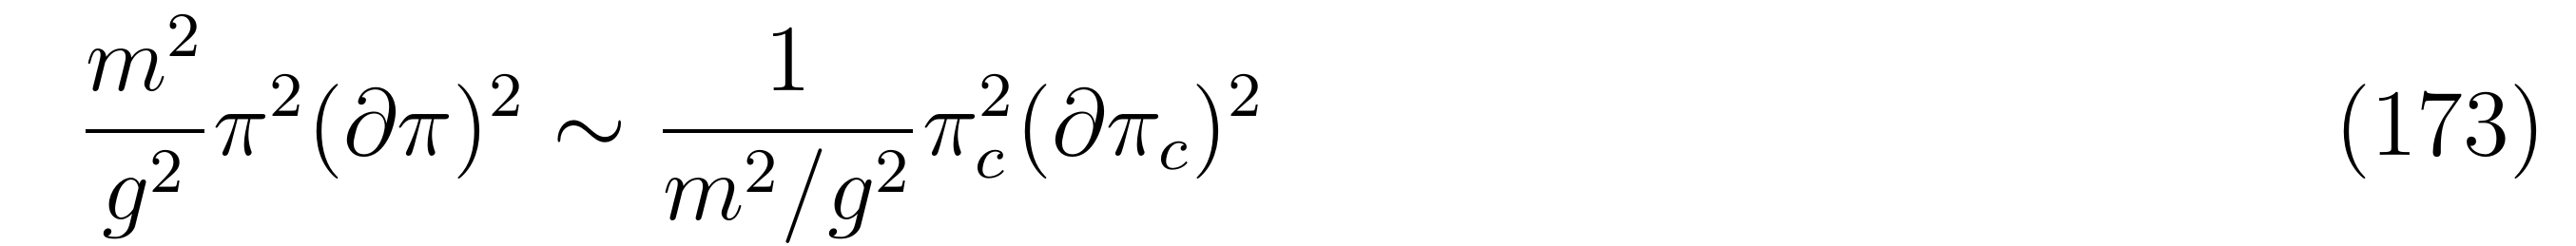
\includegraphics[width=0.677083\linewidth]{assets/eq173.png}}}
\expandafter\def\csname eq174\endcsname{\makebox[\linewidth][r]{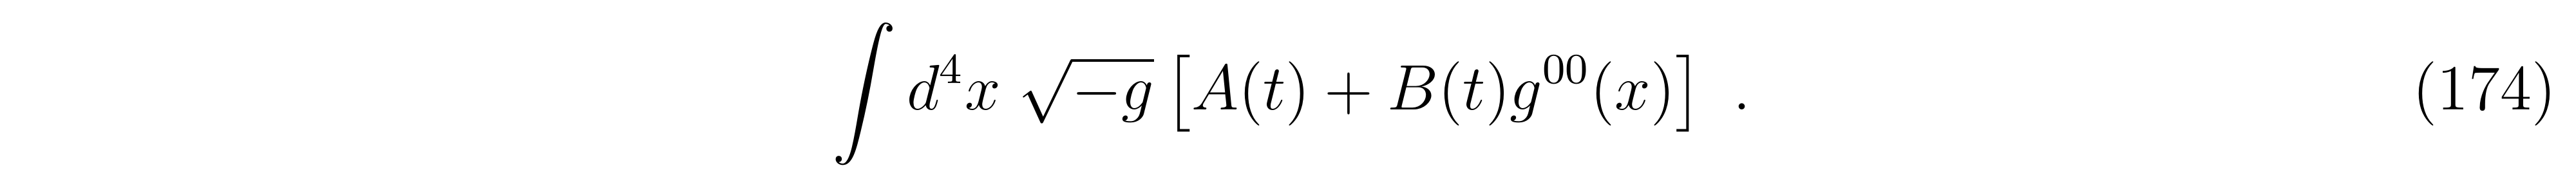
\includegraphics[width=1.000000\linewidth]{assets/eq174.png}}}
\expandafter\def\csname eq175\endcsname{\makebox[\linewidth][r]{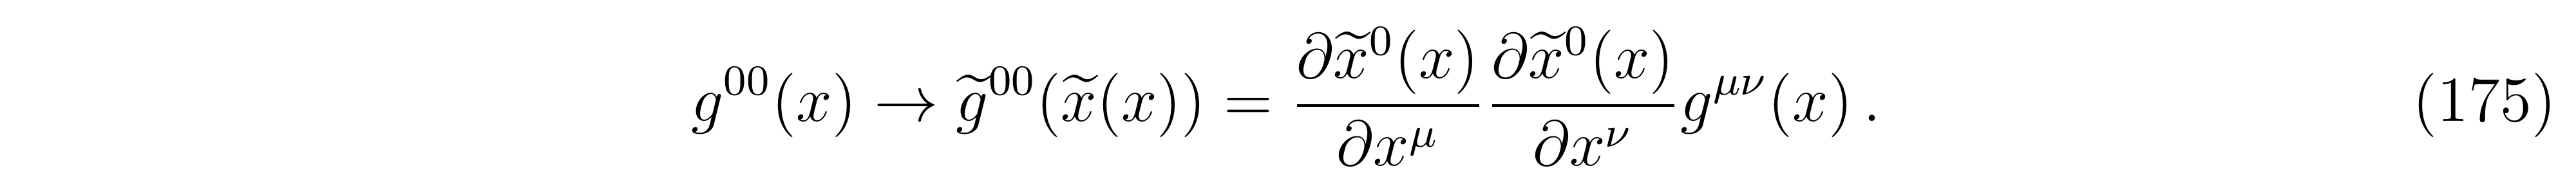
\includegraphics[width=1.000000\linewidth]{assets/eq175.png}}}
\expandafter\def\csname eq176\endcsname{\makebox[\linewidth][r]{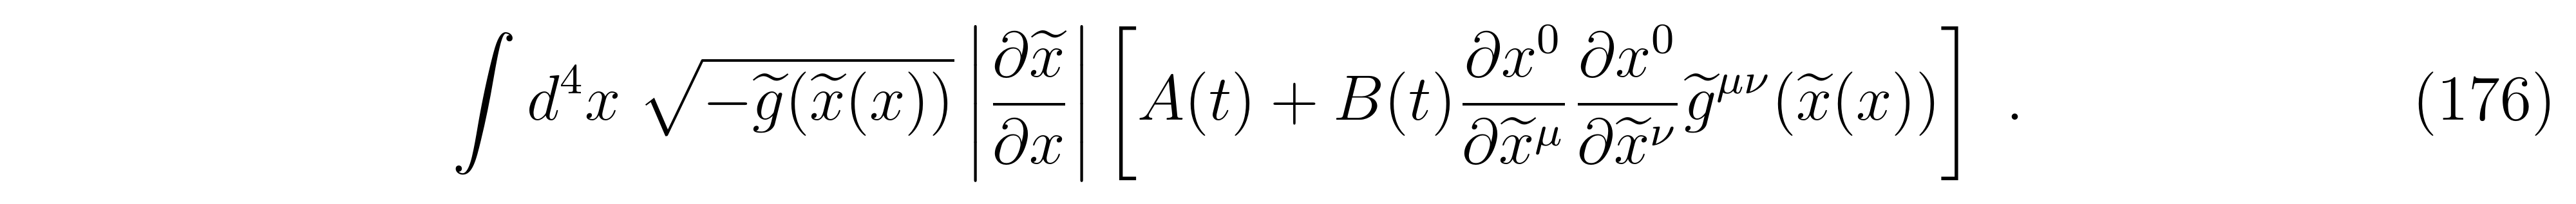
\includegraphics[width=1.000000\linewidth]{assets/eq176.png}}}
\expandafter\def\csname eq177\endcsname{\makebox[\linewidth][r]{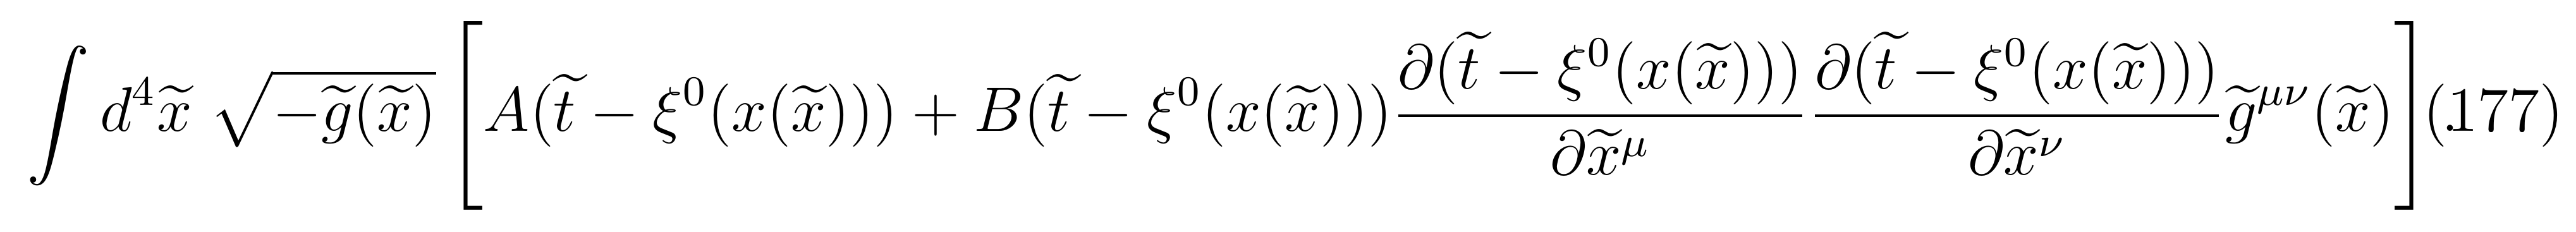
\includegraphics[width=1.000000\linewidth]{assets/eq177.png}}}
\expandafter\def\csname eq178\endcsname{\makebox[\linewidth][r]{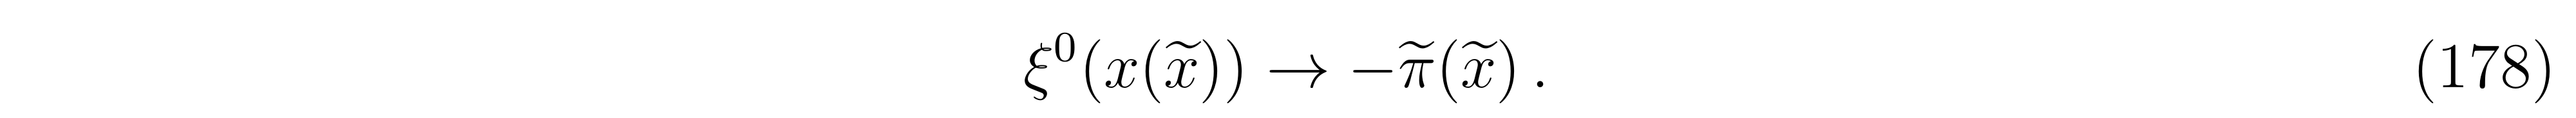
\includegraphics[width=1.000000\linewidth]{assets/eq178.png}}}
\expandafter\def\csname eq179\endcsname{\makebox[\linewidth][r]{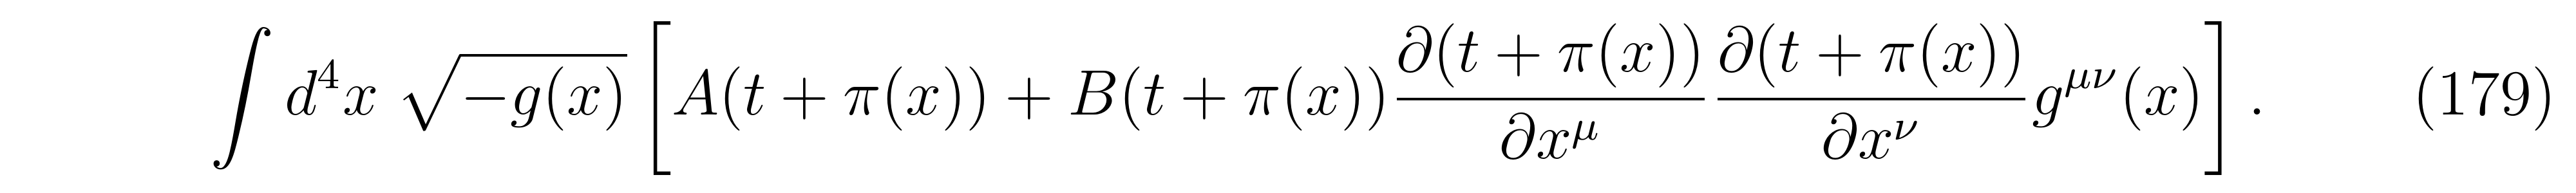
\includegraphics[width=1.000000\linewidth]{assets/eq179.png}}}
\expandafter\def\csname eq180\endcsname{\makebox[\linewidth][r]{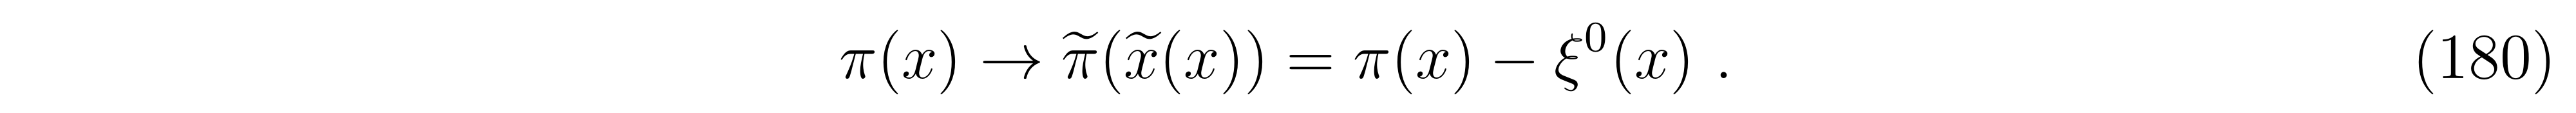
\includegraphics[width=1.000000\linewidth]{assets/eq180.png}}}
\expandafter\def\csname eq181\endcsname{\makebox[\linewidth][r]{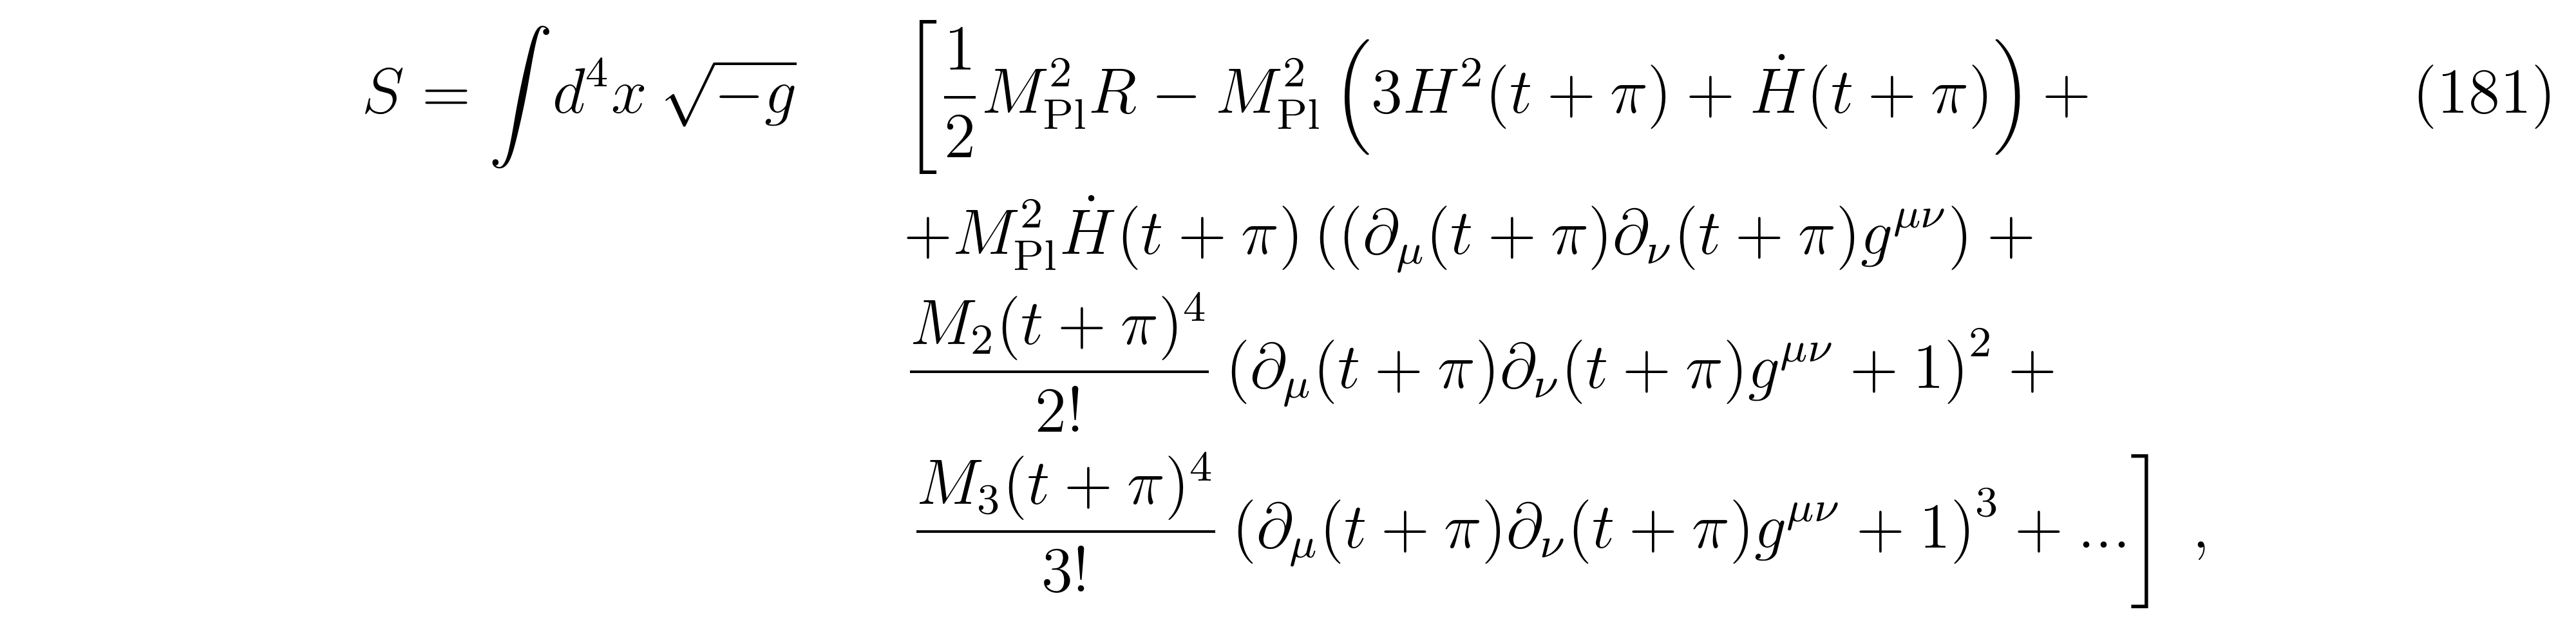
\includegraphics[width=1.000000\linewidth]{assets/eq181.png}}}
\expandafter\def\csname eq182\endcsname{\makebox[\linewidth][r]{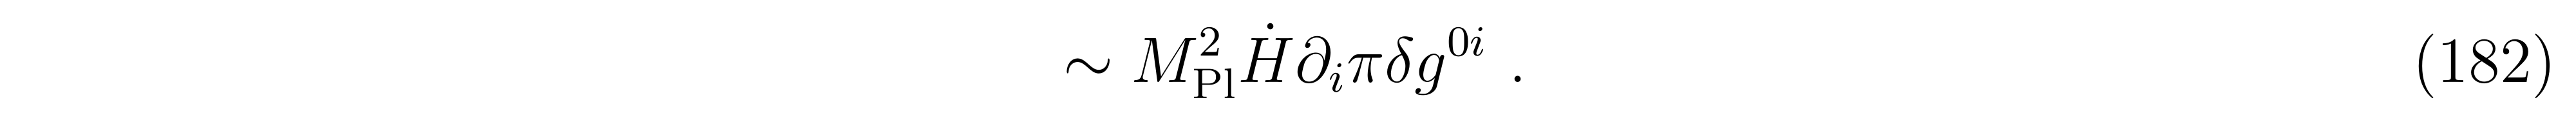
\includegraphics[width=1.000000\linewidth]{assets/eq182.png}}}
\expandafter\def\csname eq183\endcsname{\makebox[\linewidth][r]{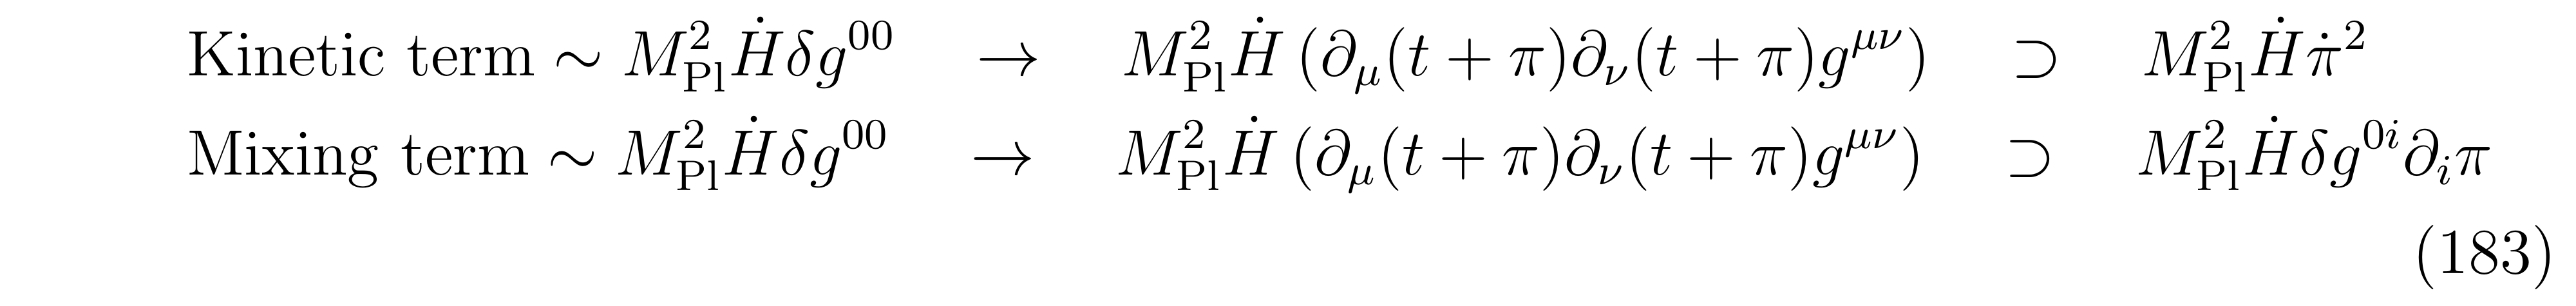
\includegraphics[width=1.000000\linewidth]{assets/eq183.png}}}
\expandafter\def\csname eq184\endcsname{\makebox[\linewidth][r]{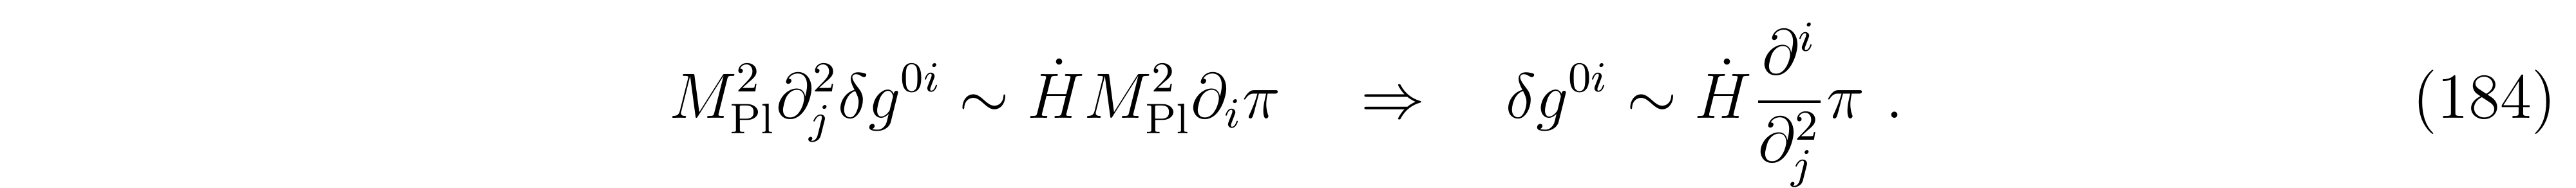
\includegraphics[width=1.000000\linewidth]{assets/eq184.png}}}
\expandafter\def\csname eq185\endcsname{\makebox[\linewidth][r]{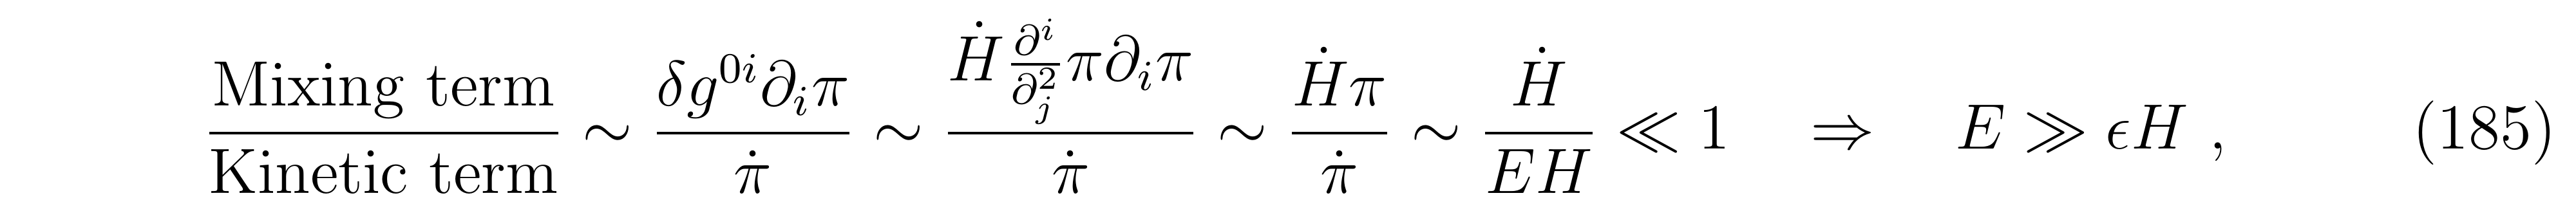
\includegraphics[width=1.000000\linewidth]{assets/eq185.png}}}
\expandafter\def\csname eq186\endcsname{\makebox[\linewidth][r]{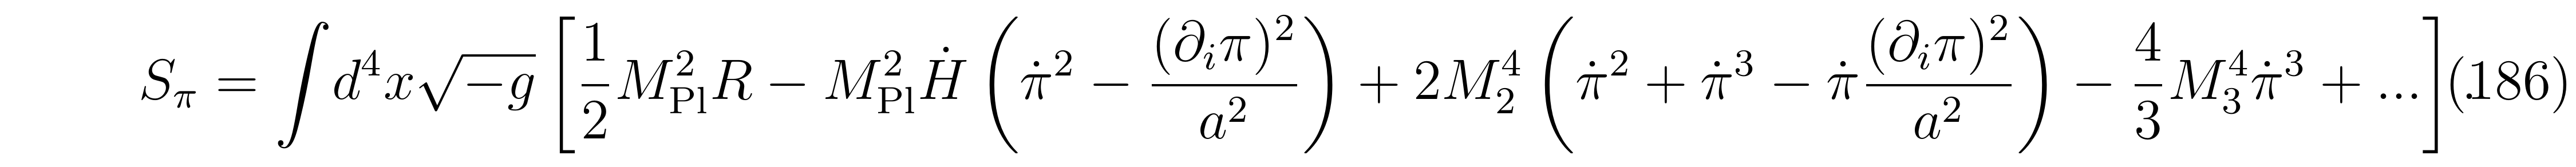
\includegraphics[width=1.000000\linewidth]{assets/eq186.png}}}
\expandafter\def\csname eq187\endcsname{\makebox[\linewidth][r]{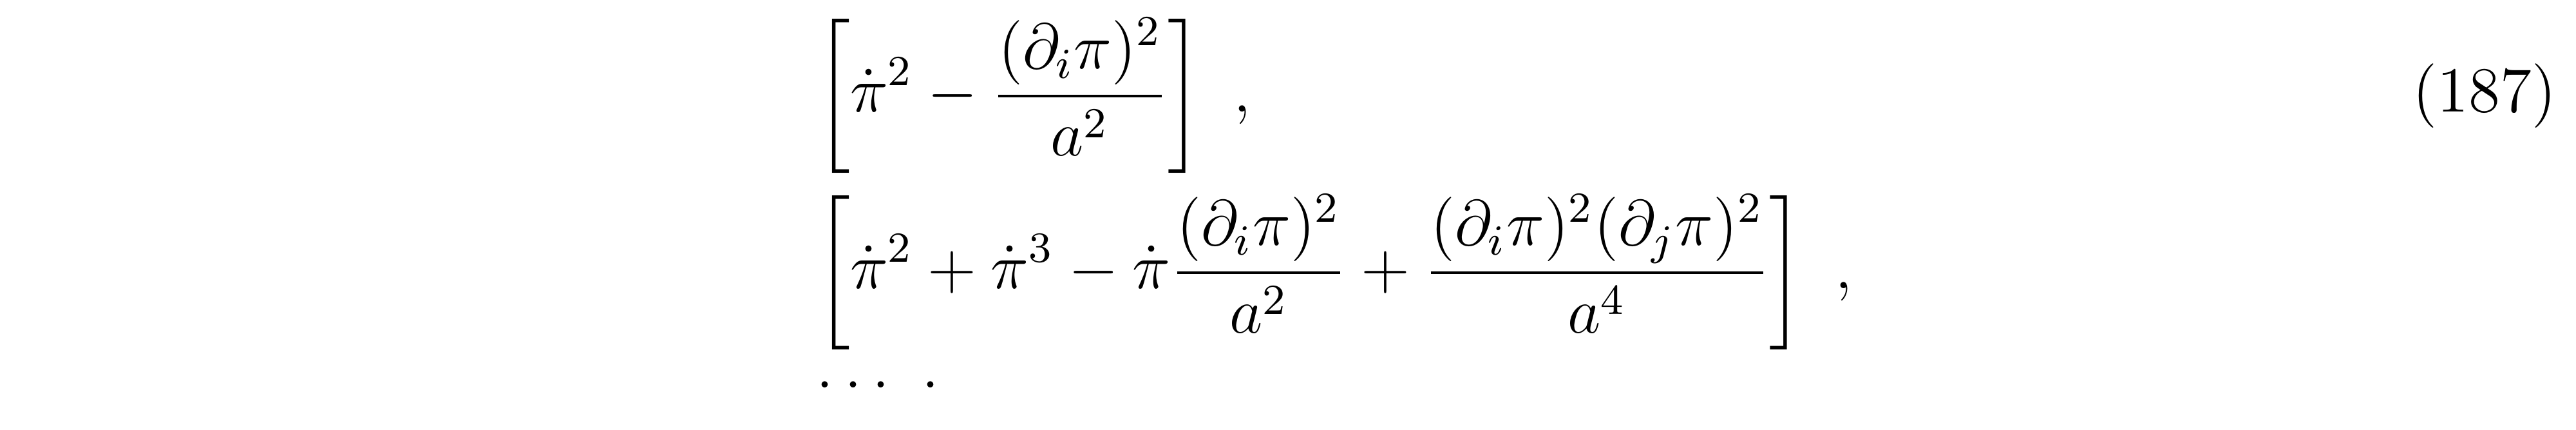
\includegraphics[width=1.000000\linewidth]{assets/eq187.png}}}
\expandafter\def\csname fig16\endcsname{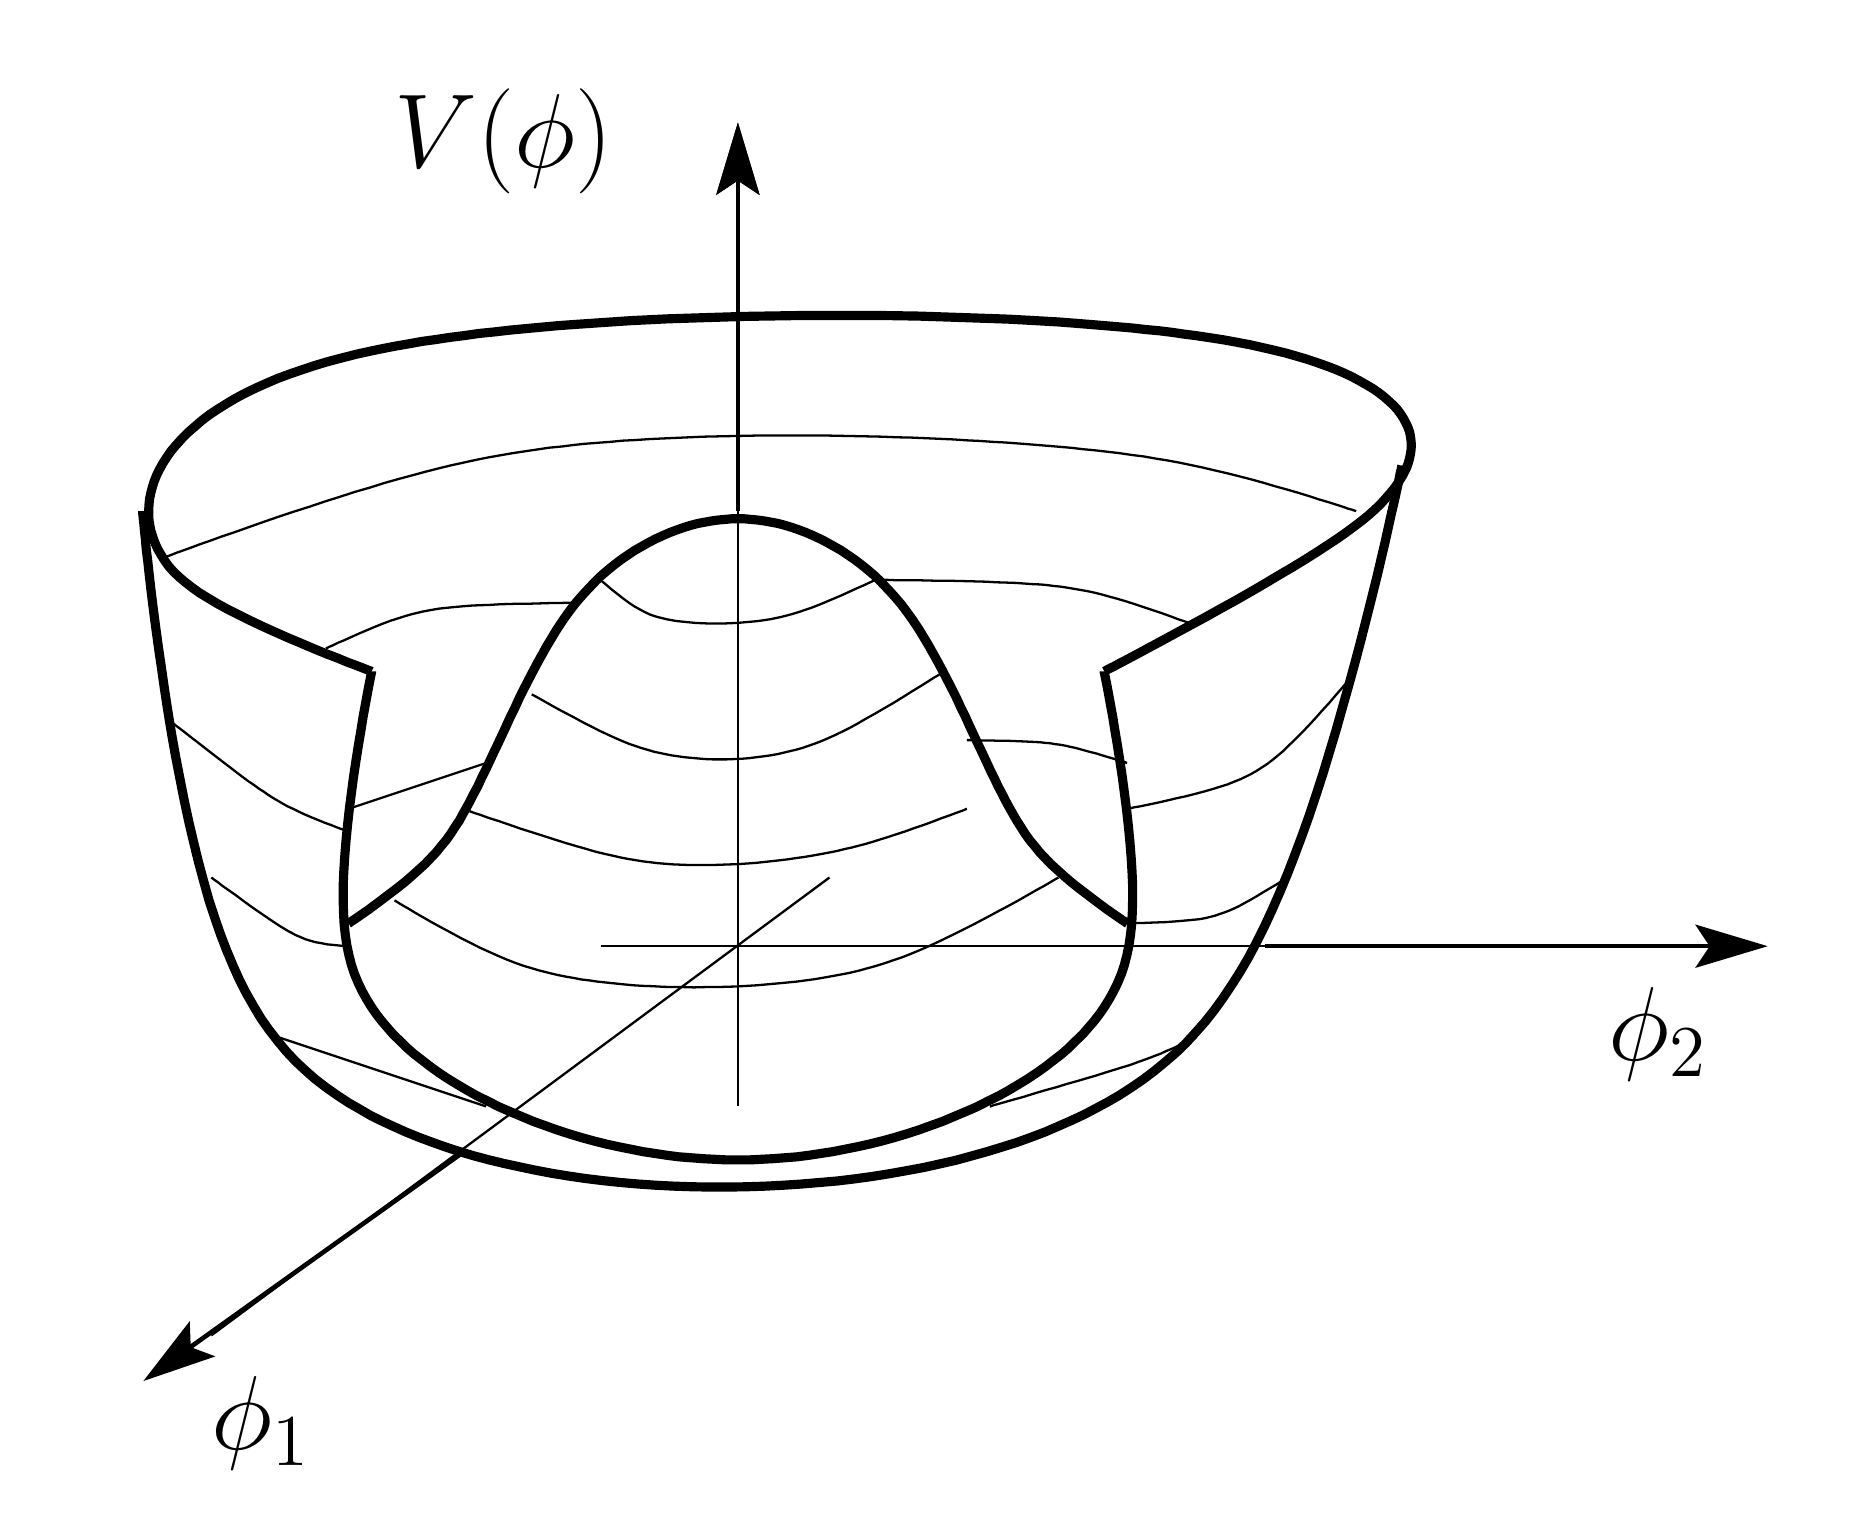
\includegraphics[width=0.48\linewidth]{assets/fig16.png}}
\expandafter\def\csname fig17\endcsname{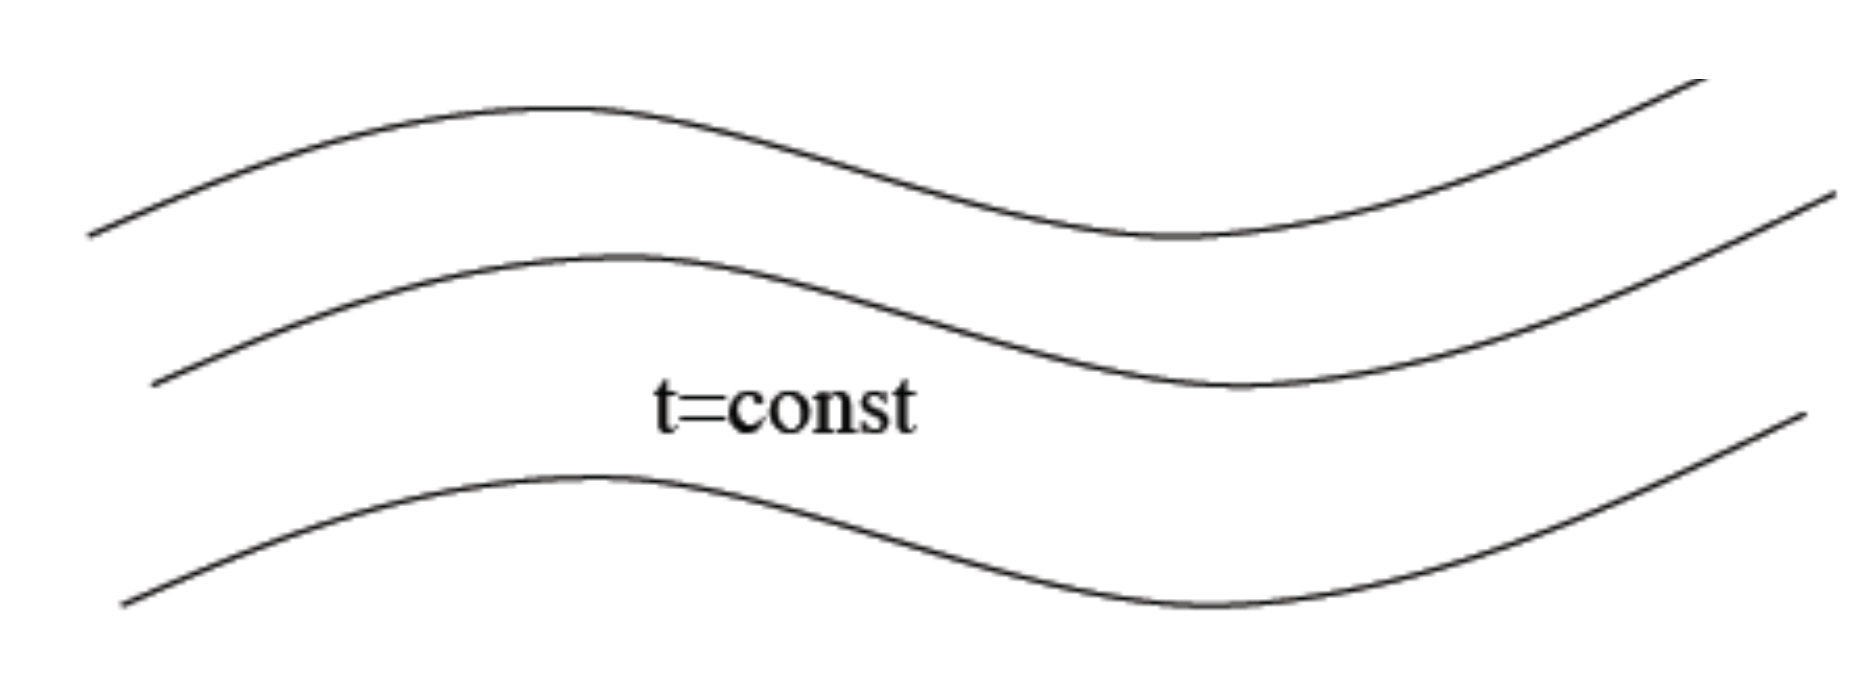
\includegraphics[width=0.48\linewidth]{assets/fig17.png}}

\title{\bfseries インフレーションの有効場理論\\[4pt]\large Lectures on Inflation §3.5 日本語訳\\[3pt]\normalsize\href{https://arxiv.org/pdf/1609.00716v1}{arXiv:1609.00716v1}}
\author{Leonardo Senatore\\\small Stanford Institute for Theoretical Physics\\\small Department of Physics, Stanford University\\\small Kavli Institute for Particle Astrophysics and Cosmology, Stanford University and SLAC}
\date{2026年10月20日}
\begin{document}
\nocite{Maldacena:2002vr,Cornwall:1974km,Cheung:2007st,Behbahani:2011it,Achucarro:2012sm,Seery:2006vu,Pimentel:2012tw,Senatore:2009cf,Senatore:2012ya}
\maketitle
\begin{abstract}
本書は、ご提供の原文PDFの第3.5節（原文40～49ページ）に基づく非公式の日本語訳である。第3.5.1節、第3.5.2節、式(151)～(187)、図16・17、脚注9～11を省略せず収録した。原論文の要旨は翻訳対象外であり、この段落は翻訳版の編集説明である。

節番号・式番号・引用番号は原文に従う。独立した数式と図は原文から生成した600dpiの高精細画像で描画を保持し、キャプションと脚注は日本語に訳した。参考文献は対象節で引用するものを原文の番号のまま収録した。原文の疑わしい表記も無断では修正していない。末尾の「原文照合について」は翻訳者による注記である。
\end{abstract}
\hypertarget{toc}{}
\tableofcontents
\clearpage
\setcounter{section}{3}
\setcounter{subsection}{4}
\subsectionlink{インフレーションの有効場理論}

有効場理論（EFT）は、素粒子物理学、さらには物性物理学においても、指導原理の役割を果たしてきた。EFTには、関心のあるエネルギースケールで重要な物理をまとめ上げる力がある。高エネルギーの、ほとんど関与しない物理の効果は、高次元演算子の係数に組み込まれる。これは、あるエネルギースケールでの現象論を探究するための方法である。これから行うのは、インフレーションの有効場理論を構築することである。その際、インフレーションをGoldstoneボソンの理論、すなわち時間並進のGoldstoneボソンの理論と捉えることができる。

\textbf{Goldstoneボソンの復習：}
Goldstoneボソンは素粒子物理学の至る所に現れる（これによってNambuは、まさに受けるに値する2008年のNobel賞を受賞した！）。メキシカンハット型のポテンシャルによって$\phi\to\langle\phi\rangle$となり、大域的な$U(1)$対称性$\phi\to e^{i\alpha}\phi$が自発的に破れる、最も単純な理論を考えよう。このとき、対称性を$\pi\to\pi+\alpha$という形で非線形に実現するGoldstoneボソン$\pi$が存在する。
\OriginalEquation{151}
したがって、場$\pi$の作用は、シフト対称性を備えた質量のないスカラー場の作用となる。
\OriginalEquation{152}
高階微分演算子は、高エネルギースケール$m/\lambda^{1/2}$の冪によって抑制される。

Goldstoneボソンの有名な例は、カイラル・ラグランジアンに現れるパイ中間子である。これは$SU(2)$カイラル・フレーバー対称性を非線形に実現するGoldstoneボソンであり、紫外（UV）側の理論であるQCDでは、クォークと反クォークの束縛状態に対応する。パイ中間子が創発的なスカラー場であることに注意しよう。QCDには基本的なスカラー場は存在しない。

\noindent\begin{minipage}{\linewidth}
\OriginalFigure{16}
\begin{center}
図16: $U(1)$対称性の自発的な破れを引き起こす、複素スカラー場のメキシカンハット・ポテンシャル。
\end{center}
\end{minipage}\par\medskip

\Needspace{4\baselineskip}
\textbf{Goldstoneボソンの理論としてのインフレーション：}
インフレーションのEFTをどのように構築すればよいだろうか。そのためには、インフレーションを最も本質的な観点から考える必要がある。インフレーションについて実際にわかっているのは、それが宇宙が準de Sitter状態にあった加速膨張の時期だということである。しかし、インフレーションは終わらなければならないので、厳密なde Sitter状態ではありえない。これは時間並進が自発的に破れていることを意味する。そこで、時間を測り、インフレーションを終わらせる物理的な時計が存在すると考えることにする。

この時計が何であろうと、一般相対論（GR）の座標不変性を利用すれば、この物理的な時計がゼロに設定される座標系へ移ることができる。任意の座標系から適切な時間微分同相変換を行い、時計の揺らぎがゼロとなる空間切片を選べばよい。例として、インフラトンが基本的なスカラー場であり（そう仮定しているわけではなく、単に例を挙げている）、$\delta\phi(\vec{x},t)\ne0$となる座標系にいるとしよう。このとき、次式が成り立つように時間微分同相変換$t\to\tilde{t}=t+\delta t(\vec{x},t)$を行うことができる（ここでは線形次数で示すが、任意の非線形次数へ一般化できる）。
\OriginalEquation{153}
さて、この座標系にいるとしよう。EFTの規則に従うことにする。その規則によれば、利用可能な自由度を用いて作用を書かなければならない。ここでは、それは計量の揺らぎだけである。揺らぎについて展開し、この問題の対称性と両立するすべての演算子を書き下さなければならない。今の場合、さまざまな空間切片の内部で空間座標を任意に変えることができ、それぞれの空間切片で異なる変換をしてよい。このことは、残るゲージ対称性が時間に依存する空間微分同相変換であることを意味する。
\OriginalEquation{154}

さらに、引き続きEFTの手順に従って、摂動について関心のある次数まで展開する（例えば、2点関数には2次、3点関数には3次、4点関数には4次、という具合である）。そのうえで、揺らぎの各次数において微分について展開する。高階微分項は、この問題のエネルギースケール$E$と何らかの高エネルギースケール$\Lambda$との比によって抑制される。

\noindent\begin{minipage}{\linewidth}
\OriginalFigure{17}
\begin{center}
図17: インフレーションを駆動する時計場が存在するならば、この時計を一様とする、特別な時間切片の取り方が存在する。
\end{center}
\end{minipage}\par\medskip

\subsubsection{ユニタリーゲージにおける作用の構成}

このユニタリーゲージで最も一般的なラグランジアンは何だろうか。ここでは文献\cite{Cheung:2007st}にほぼ沿って議論する。計量$g_{\mu\nu}$の関数であり、（線形に実現される）時間に依存する空間微分同相変換$x^i\to x^i+\xi^i(t,\vec{x})$のもとで不変な演算子を書き下さなければならない。時間に依存する空間微分同相変換は、実際、破れていない。言葉でいえば、インフレーションとは、時空の微分同相変換が時間に依存する空間微分同相変換へと自発的に破れた理論だということである\footnote[9]{微分同相変換はゲージの冗長性であることを覚えておこう（ゲージ対称性と呼ばれることもあるが、この呼び方はやや誤っている）。この点でインフレーションの理論は、$SU(2)\times U(1)$のゲージの冗長性が$U(1)$のゲージの冗長性へと自発的に破れる、低エネルギーでの素粒子物理学の標準模型に類似している。}。すべての微分同相変換に対して不変な、Riemannテンソルを含む通常の項に加えて、この系では対称性が減少しているため、多数の追加の項が許されるようになる。これらは、重力子に吸収された追加の自由度を記述する。例えば、$g^{00}$が空間微分同相変換のもとでスカラーであることは容易にわかる。したがって、ユニタリーゲージのラグランジアンには$g^{00}$が自由に現れてよい。
\OriginalEquation{155}
微分を含まない項は、$g^{00}$の多項式だけである。時空に特別な切片の取り方が存在するので、その切片を記述する幾何学的な量を書き下すことも許される。例えば、等時刻面の外部曲率$K_{\mu\nu}$は空間微分同相変換のもとでテンソルであり、作用に用いることができる。$n^\mu$を等時刻切片に直交するベクトルとすると、
\OriginalEquation{156}
である。ここで、$\nabla$は共変微分、$h_{\mu\nu}$は空間切片上の誘導計量であり、
\OriginalEquation{157}
と表される。

作用のどの項にも、一般の時間の関数を掛けてよいことに注意しよう。最も一般的なラグランジアンは、次のように書ける（証明は文献\cite{Cheung:2007st}の付録AおよびBを参照）。
\OriginalEquation{158}
ここで、省略記号は、揺らぎについてより高次の項、あるいはより多くの微分を含む項を表す。また、$\delta g^{00}=g^{00}+1$である。$\delta K_{\mu\nu}$は、等時刻面の外部曲率の、摂動のないFRWに対する変化を表し、$\delta K_{\mu\nu}=K_{\mu\nu}-a^2Hh_{\mu\nu}$である。ここで$h_{\mu\nu}$は誘導された空間計量である。上の作用において、選んだFRW解のまわりの線形摂動を含むのは最初の3項だけであり、その他はすべて明示的に2次以上であることに注意しよう。したがって、係数$c(t)$と$\Lambda(t)$は、与えられたFRWの発展$H(t)$をもつという要請、すなわち、この解のまわりでタドポール項が相殺されるという要請によって決まる。これらの係数を決定する前に、この簡略化が自明でないことを理解しておくことが重要である。背景解のまわりの1次で寄与する演算子は無限に多数あると考えられるだろう。しかし、$\delta K_{\mu\nu}$や$g^{00}+1$のような線形項の多項式として作用を書けば、ある演算子が1次、2次、あるいはさらに高次のどこから始まるかが明らかになる。式\eqref{eq:158}にあるもの以外のすべての線形項は微分を含み、部分積分によって、ここで考えた3つの線形項と、高次の共変な項との組み合わせにできる。したがって、\emph{摂動のない発展の履歴によって$c(t)$と$\Lambda(t)$が決まり、異なる模型間の違いは高次の項に組み込まれる}と結論できる。

ここで、与えられたFRWの発展が解となることを要求して、線形項を決定できる。すでに述べたように、$c$と$\Lambda$に比例する項だけが、エネルギー運動量テンソル
\OriginalEquation{159}
に、摂動の0次で消えない寄与を与え、したがってEinstein方程式の右辺に寄与する。インフレーションの間に主として関心があるのは、平坦なFRW宇宙
\OriginalEquation{160}
なので、Friedmann方程式は次のようになる。
\OriginalEquation{161}
\OriginalEquation{162}

$c$と$\Lambda$について解くと、作用\eqref{eq:158}を次のように書き換えられる。
\OriginalEquation{163}
すでに述べたように、上の作用に含まれる演算子の係数は、すべて一般の時間依存性をもってよい。しかし、ここで関心があるのは、1 Hubble時間の間に$H$と$\dot H$が大きく変化しない解である。したがって、他のすべての演算子についても同じことが成り立つと仮定するのが自然である。この仮定のもとでは、ラグランジアンは近似的に時間並進不変となる\footnote[10]{時間シフトが厳密な対称性となる極限は、$\dot H\to0$となるため、注意して取らなければならない。これは、ゴースト・インフレーションの議論で見るように、Goldstoneの空間的な運動項が消えることを意味する。}。そのため、ループ効果によって生じる時間依存性は、小さな対称性の破れのパラメーターによって抑制される\footnote[11]{この対称性は、時間微分同相変換の破れとは無関係であることに注意しよう。この対称性が$\phi$を用いた記述でどのように現れるかを見るには、適切な場の再定義を行えば、常に$\dot\phi=\mathrm{const.}$と仮定できることに注目するとよい。このように選ぶと、シフト対称性$\phi\to\phi+\mathrm{const.}$から、ユニタリーゲージのラグランジアンの時間並進不変性が従う。この対称性と、$\phi$のラグランジアンの時間並進対称性は、背景によって対角部分群へと破れる。この残った対称性が、ユニタリーゲージのラグランジアンにおける時間シフトである。}。この仮定は特に都合がよい。というのも、係数の急速な時間依存性は、指数関数的な膨張によって生じる摩擦に打ち勝つことがあり、その場合、インフレーションが力学的なアトラクターではなくなりうるからである。力学的なアトラクターであることは、標準的なFRW宇宙論の一様性問題を解決するために必要である。

このアプローチが、スカラーモードだけでなく重力についても最も一般的なラグランジアンを記述していることを強調しておきたい。例えば、高エネルギーの効果は、Riemannテンソルの摂動$\delta R_{\mu\nu\rho\sigma}$を含む演算子に組み込まれる。これらの補正は微分について高次なので、以下では明示的には議論しない。

単純なインフレーション模型をこの言葉でどのように書くか、いくつか例を挙げよう。最小の運動項とスローロール・ポテンシャル$V(\phi)$をもつ模型は、ユニタリーゲージでは次のように書ける。
\OriginalEquation{164}
Friedmann方程式から$\dot\phi_0(t)^2=-2M_P^2\dot H$および$V(\phi(t))=M_{\mathrm{Pl}}^2(3H^2+\dot H)$が得られるので、この作用は、最初の3項以外をすべてゼロとした式\eqref{eq:163}の形であることがわかる。明らかに、これが厳密に成り立つことはありえない。他のすべての項はループ補正によって生成されるからである。それらの項には、この単純なスローロール・インフレーション模型に対する、高エネルギーの物理のありうるすべての効果が組み込まれている。

より一般的な場合には、それぞれの$\phi$に作用する微分が高々1つであるような、ありうるすべてのラグランジアンが含まれる。すなわち、$\mathcal{L}=P(X,\phi)$であり、ここで$X=g^{\mu\nu}\partial_\mu\phi\partial_\nu\phi$である。摂動のない解$\phi_0(t)$のまわりでは、
\OriginalEquation{165}
となる。これは明らかに上記の形であり、$M_n^4(t)=\dot\phi_0(t)^{2n}\partial^nP/\partial X^n$を$\phi_0(t)$において評価したものとなっている。外部曲率を含む項は、1つのスカラーに作用する微分を2つ以上含み、厳密なde Sitter極限$\dot H\to0$において決定的に重要となる。これらはゴースト・インフレーションと、この枠組みで発見される新しい模型を再現する。

\subsubsection{Goldstoneボソンの作用}

ユニタリーゲージのラグランジアンは非常に一般的であるが、明らかにあまり直観的ではない。例えば、ある特定の極限では標準的なスローロール・インフレーションを含む。しかし、スカラーの自由度はどこにあるのだろうか。これほど複雑なのは、これが自発的に破れたゲージ対称性のユニタリーゲージでのラグランジアンだからである。

\noindent\textbf{Goldstoneボソンの等価定理：}
ユニタリーゲージのラグランジアンは、重力子の二つのヘリシティーと一つのスカラーモードという三つの自由度を記述する。このモードは、破れた時間の微分同相変換を行うことにより（Stückelbergの手法）、この対称性を非線形に実現するGoldstoneボソンとして明示的に現れる。質量をもつゲージボソンの縦成分に関する等価定理\cite{Cornwall:1974km}との類推から、混合を無視できる短距離では、Goldstoneボソンの物理は重力子の二つのヘリシティーから分離すると期待される。同じ方法をわれわれの場合に適用する前に、非Abelianゲージ理論で何が起こるかを簡単に復習しよう。

非Abelianゲージ群の$A_\mu^a$に対するユニタリーゲージの作用は
\OriginalEquation{166}
である。ここで$A_\mu=A_\mu^aT^a$である。ゲージ変換の下で
\OriginalEquation{167}
となる。したがって作用は
\OriginalEquation{168}
となる。質量項はゲージ不変ではなかったため、この項には$U$の因子が現れる。$U=\exp[iT^a\pi^a(t,\vec{x})]$と書くことにより、ゲージ不変性を「回復」できる。ここで$\pi^a$はスカラー（Goldstoneボソン）であり、ゲージ変換$\Lambda$の下で
\OriginalEquation{169}
のように非線形に変換する。

ここで一時的に、ゲージ理論が$U(1)$理論である場合を考えると、
\OriginalEquation{170}
となることに注意しよう。$\pi$はゲージ変換の下でシフトする。$0$が$0$へ写されないので、これは非線形変換である。非線形に変換する力学的な場を再導入することによって、ゲージ不変性が回復された。ゲージ不変性は非線形に実現されている。

正準規格化に移ると、
\OriginalEquation{171}
Goldstoneボソンの自己相互作用は、ゲージボソンの質量よりもパラメトリックに高いスケール$4\pi m/g$で強結合になることが分かる。Goldstoneボソンを再導入する利点は、エネルギー$E\gg m$では、Goldstoneボソンとゲージ場の横成分との混合が重要でなくなり、両者のセクターが分離することである。実際、式\eqref{eq:167}の混合項は
\OriginalEquation{172}
という形であり、$E\gg m$では正準運動項$(\partial\pi_c)^2$に比べて重要でない。

$D_\mu U D^\mu U$という項を展開すると、
\OriginalEquation{173}
という形の非関連な（すなわち繰り込み不可能な）項が得られることに注意しよう。これは、エネルギー$E\sim4\pi m/g$で強結合になり、ユニタリー性の破れを引き起こす演算子である。

$m\ll E\ll4\pi m/g$の範囲では、Goldstoneボソン$\pi$の物理は弱結合であり、横成分との混合を無視して調べることができる。

われわれが扱う、時間の微分同相変換が破れた場合について、同じ手順をたどろう。例えば、次の二つの演算子に注目しよう。
\OriginalEquation{174}
破れた時間の微分同相変換$t\to\tilde{t}=t+\xi^0(x)$、$\vec{x}\to\tilde{\vec{x}}=\vec{x}$の下で、$g^{00}$は次のように変換する。
\OriginalEquation{175}
変換後の場を用いて書いた作用は、次のようになる。
\OriginalEquation{176}
積分変数を$\tilde{x}$に変えると、次を得る。
\OriginalEquation{177}
Goldstoneボソンを再導入する手順は、ここでもゲージ理論の場合と同様である。上の作用に$\xi^0$が現れる箇所ではすべて、次の置き換えを行う。
\OriginalEquation{178}

これにより、簡単のためチルダを省略すると、次を得る。
\OriginalEquation{179}
\(\pi\) に変換則
\OriginalEquation{180}
を与えれば、上の作用が、無限小変換に限らず、あらゆる次数で微分同相変換に対して不変であることを確かめられる。この定義では、時間の微分同相変換のもとで、\(\pi\) はスカラー場としての変換に加えてシフトを受ける。もともと微分同相不変な項には \(\pi\) が現れないことに注意しよう。

この手続きをユニタリーゲージの作用\eqref{eq:163}に適用すると、
\OriginalEquation{181}
を得る。ここではひとまず、簡単のため外部曲率を含む項を無視した。

この作用はかなり複雑であり、この段階では、ユニタリーゲージのラグランジアンからGoldstoneボソン \(\pi\) を再導入する利点は明らかではない。ゲージ理論の場合と同様、十分短い距離では計量の揺らぎを無視してGoldstoneボソンの物理を調べられるため、簡単化が生じる。これはまさに等価原理である。ゲージ理論の場合と同じく、それが可能となる領域は、上のラグランジアンの混合項を見るだけで見積もることができる。実際、式\eqref{eq:181}では、\(\pi\) と \(g_{\mu\nu}\) を混合する二次の項は \(\pi\) の運動項よりも微分の数が少なく、ある高いエネルギースケールを超えると無視できる。一般には、その答えはどの演算子が存在するかに依存する。ここでは、タドポール項だけが重要な最も簡単な場合、\(M_2=M_3=\cdots=0\) を考えよう。これは標準的なスローロール・インフレーションを含む。重力との主要な混合は、次の形の項から生じる。
\OriginalEquation{182}
次が成り立つことが分かる。
\OriginalEquation{183}
\trnote{式中の Kinetic term は運動項、Mixing term は混合項を表す。}

\(\delta g^{0i}\) は拘束変数であり、ある種の重力ポテンシャルに相当し、\(\pi\) によって決まる。短距離ではNewton近似が成り立つ。
\OriginalEquation{184}
したがって、
\OriginalEquation{185}
となる。最後から二番目の段階では空間微分について部分積分を行い、最後の段階では、エネルギーが \(E\) 程度のとき \(\partial_t\sim E\) であることを用いた。混合項は紫外領域で無視できる。これは一般相対論の等価原理である。混合を無視できるようになる実際のスケール \(E_{\mathrm{mix}}\) は、どの演算子を非零とするかに依存するが、エネルギー \(E\gg E_{\mathrm{mix}}\) では混合項を無視できることが保証される。

\(E\gg E_{\mathrm{mix}}\) の領域では、作用は劇的に簡単になり、
\OriginalEquation{186}
となる。
時間の微分同相変換が非線形に実現されることにより、\(\pi\) は非線形な「ブロック」
\OriginalEquation{187}
の形で現れなければならないことに注意しよう。これにより、異なる演算子の間に厳密な関係が与えられる。

あるインフレーション模型が与えられたとき、関心があるのは現在の宇宙論的観測に対する予言を計算することである。この観点から見ると、分離極限\eqref{eq:186}は、このような極端に赤外のスケールとはまったく関係がないように思われる。しかし、標準的な単一場のスローロール・インフレーションの場合と同様、通常の \(\zeta\) 変数という量が存在し、それが地平線の外側では摂動論の任意の次数で一定となることを証明できる。

したがって、問題は地平線通過の直後の相関関数を計算することに帰着する。このため、\(H\) 程度の赤外エネルギーカットオフを設けてラグランジアンを調べればよい。分離のスケール \(E_{\mathrm{mix}}\) が \(H\) より小さければ、\(\pi\) のラグランジアン\eqref{eq:186}は、\(E_{\mathrm{mix}}/H\) で抑制される項を除いて正しい予言を与える。そうでない場合にも、何か深刻なことが起こるわけではない。単に計量の揺らぎも保持すればよい。

これが、第2講で行った計算の正当化である。

すでに述べたように、ユニタリーゲージのラグランジアンの係数の時間変化はHubble時間に比べて緩やかである、すなわち何らかの一般化されたスローロール・パラメーターによって抑制されていると仮定している。このことは、係数のTaylor展開から生じる追加の \(\pi\) の項が小さいことを意味する。特に、三次の項のような関連演算子、すなわち赤外へ向かうにつれて支配的になる演算子は、スケール \(H\) では重要ではないため、ラグランジアン\eqref{eq:186}では無視した。それでも、文献\cite{Behbahani:2011it,Achucarro:2012sm}で行われているように、これらを取り入れることは容易である。

結論として、ラグランジアン\eqref{eq:186}を用いると、重力との混合が支配的ではないすべての観測量、例えば標準的なスローロール・インフレーションにおける非Gaussian性\cite{Maldacena:2002vr,Seery:2006vu}などを計算できる。ただし、スペクトルの傾きは、主要次数ではラグランジアン\eqref{eq:186}を用いて計算できる。先に見たように、その値は、混合項を無視して計算した地平線通過時のパワースペクトルから簡単に求められる。重力との混合が重要になり、Goldstoneボソンの作用だけでは予言に十分でなくなった場合でも、このアプローチの妥当性が失われるわけではないことを強調しておく。作用\eqref{eq:163}には模型に関するすべての情報が含まれており、重力との混合が大きい場合にも、あらゆる予言を計算するために用いることができる。

いくつかの点を強調しておこう。
\begin{itemize}
\item 上のラグランジアンは非常に簡単であり、単一の自由度をもつインフレーション模型をすべて統一的に記述する。
\item これは揺らぎの理論を記述する。そして、実際に検証しているのはその揺らぎである。
\item 素粒子物理学のカイラルラグランジアンに対応するものである。実際、実験の観点から見れば、インフレーションはGoldstoneボソンの理論であることを示している。
\item 単一の時計をもつインフレーション模型をすべて包含しているため、可能なシグナルについての定理を証明できる。
\item また、考えられるあらゆるシグナルを調べることができる。
\item 対称性によって何が強制され、どの演算子が許され、何が可能なのかが明確になる。例えば、\((\partial_i\pi)^2\) の係数は \(\dot H M_{\mathrm{Pl}}^2\) に固定される。\(\dot\pi^2\) についてはそうではない。このことは、微分の主要次数ではヌル・エネルギー条件を破れないことを意味する。\(\dot H>0\) であれば、\(\pi\) の空間的な運動項の符号が負のエネルギーに対応するものとなり、制御不能な不安定性をもたらす。EFTは、高階微分項を加えることによってこの問題をどのように解決できるかも教えてくれる。実際、現在知られているヌル・エネルギー条件（NEC）を破る方法は、すべてこの枠組みの中で見いだされたものである。
\item この形式は、標準模型を超える物理で通常行うことを実践するのに適している。対称性を加えて、ある演算子をほかの演算子に比べて増強することもできるし、特定の模型の紫外完備化を試みることもできる。
\item 明示的に揺らぎの理論であるため、演算子の重要性を容易に評価できる。例えば、スカラー場を用いた標準的な扱いでは、演算子 \((\partial\phi)^8\) は、\(\dot\phi_0^6(\partial\delta\phi)^2\) を通じて二次の作用に寄与する。この点はループ補正を調べるうえでも非常に有用である。揺らぎと微分の次数を固定すると、EFTには有限個の相殺項しか存在しないが、スカラー場の理論ではそうではない。実際、EFTの形式は、量子レベルでの \(\zeta\) の一定性を証明するために不可欠であった\cite{Pimentel:2012tw,Senatore:2012ya}。
\end{itemize}

\clearpage
\phantomsection
\addcontentsline{toc}{section}{原文照合について}
\section*{\hyperlink{toc}{原文照合について}}
\noindent 以下は原文の本文とは別の翻訳上の注記である。
\begin{itemize}
\item 式(156)の添字と、式(158)直後の $\delta K_{\mu\nu}=K_{\mu\nu}-a^2Hh_{\mu\nu}$ の表記は原文のまま保持した。
\item 式(164)直後の本文の $M_P$、式(165)の $\phi(t)$、式(173)直前の本文の $D_\mu U D^\mu U$、式(185)の分母・係数なども、原文に示された表記を保持した。
\item 原文49ページの結論段落では、「重力との混合が支配的ではない観測量」と「標準的なスローロール・インフレーションの非Gaussian性」の例示との関係に解釈の余地がある。本文は文面に沿って訳し、例外であるとの解釈を補っていない。
\item 参考文献[28]は原文で2件の論文をまとめた項目であるため、ここでも同じ番号に2件を収録した。
\end{itemize}
\noindent\textbf{出典とライセンスの確認：}
原著は Leonardo Senatore, \textit{Lectures on Inflation}, \href{https://arxiv.org/pdf/1609.00716v1}{arXiv:1609.00716v1} である。\href{https://arxiv.org/abs/1609.00716v1}{arXiv掲載ページ}が示すライセンスは、\href{https://arxiv.org/licenses/nonexclusive-distrib/1.0/license.html}{arXivの非独占的配布ライセンス}である。このライセンスから第三者への翻訳・再配布の許諾は確認できなかった。本訳は利用者から提供されたPDFを対象として作成した。

\newpage
\renewcommand{\refname}{\hyperlink{toc}{参考文献}}

\bibliographystyle{utphys}
\bibliography{ref}
\end{document}
